

\section{Introduction}
\subsection{Introduction to General Relativity}
general gr shit?
mention einstein derivation (hilbert derivation a potentially earlier but vacuum), karl schwarzshild ( ironicaly meaning black shield), then low mass limit, photon deflection and mercury perihelion around sun. mention cosmology, gravitational waves, more black holes, minkowski. more compact objects. 

The modern theory of gravity, published by Albert Einstein in 1915, is general relativity (GR). It is a geometric theory relying on curved spaces and differential geometry. GR is a generalisation of Einstein's theory of special relativity (SR) to include matter and gravity. Where the main idea behind SR was that the laws of physics are identical in any non-accelerating frame, GR includes the gravitational force (and subsequently matter) by postulating that the laws of phsyics are identical in any free-falling frame. In a universe without gravity or matter, also called a vaccum universe, GR is equivalent to SR.

GR also supercedes Newton's theory of gravity when gravity becomes stronger. In Newtonian theory, two masses orbit each other in a constant circle or ellipse; the ellipses can precess in the presence of extra masses. However, the calculated precession rate of Mercury about the sun using Newton's theory of gravity was much to slow; Einstien correctly calculated the precession rate using GR. This initial success proved to the world that Einstein's theory was the best current describtion of gravity. In the weak gravity limit, GR perfectly replicates Newton's theory of gravity; the precession of Mercury is the most stark deviation from Newton's theory as it is closest to the sun where gravity is the strongest. 

Other new effects predicted by GR including gravitational time dilation and light ray deflection. Gravitational time dilation is similar to time dilation in SR which states that an observer at rest would age more quickly (in their own frame) compared to a quickly moving observer. Gravitational time dilation states that an observer in a stronger gravitational field will age slower than one in a weaker gravitational field; this effect has been verified by comparing two atomic clocks where one is left on the surface of the earth and one is elevated. Light ray deflection occurs when a beam of light passes close by an object with a strong gravitational field - the stronger the field the more the light beam is deflected. This can be seen when distant bright objects pass behind matter, for example black holes or even the sun.

In the moderately strong gravity regime, Newtons theory starts to become quite innacurate. After many orbits of two (or more) heavy objects the time averages separtion can be seen to decrease, hence the objects are inspiralling. The orbital energy lost is released as a gravitational wave (GW) signal. Inspiralling and radiation becomes more pronounced at lower separtions and with heavier objects. If the inspiralling becomes significantly fast compared to an orbit time, then Newton's theory of gravity can fail to accurately simulate the binary; approxiations to GR can be used in this regime, for example post newtonian (PN) theory.

In the strong gravity regime GR deviaties entirely from Newtonian theory leading to a plethora of exotic results. One example is the neutron star (NS), an object so dense that all of the electons in an atom are forced to combine with nearby protons and reduce all matter to a dense lattice of neutrons. The gravitational field on the surface of a NS is of order $10^{11}$ times stronger than on earth. Another example is the black hole (BH), an even denser object with such a strong gravitational pull that even light cannot escape. These dense objects can be produced by the collapse of large dying stars, implosions of supernovae, and collisions of very dense objects.

At the centre of a black hole, GR predicts a singularity; a single infinitely dense point surrounded by vacuum. it is presumed that Einstein's theory breaks down towards a singularity which is deemed unphysical. Theories such as loop quantum gravity (LQG) and string theory (ST) try to reconcile GR with quantum mechanics which is thought might aleviate this problem. Sadly there is no definive answeras to what happens near a gravitational singularity, this is in part due to the lack of experimental data to draw from. The weak cosmic sensorship hypothesis states that all physical singularities are hidden inside an event horizon; a surface which contains all points that are cannot send information to an observer infinitely far away in the infinite future. This is called causally disconnected. 

Black holes in the universe generally spin, this is due to any black hole forming from the collapse of matter will inherit the angular momentum of the matter as it collapses. Rotating black holes were first described by Roy Kerr in 1963, and therefore are called Kerr black holes. The collisions of black holes (with or without spin) is also successfully described by GR, however this phenomenon is far too complicated to solve analytically. Numerical relativity (NR), the exact simulation of GR using methods to solve partial differential equations (PDEs), is needed to describe black hole collisions and inspirals. 

GR also describes physics at the largest scales, not just compact regions and objects as discussed so far. The application of GR to the entire universe is called Cosmology. Cosmology can be used to describe the big bang, early universe expansion, and late universe inflation. Cosmology can also be used to describe a universe with small matter and gravitational perturbations ontop of a uniform background, this is the best current description of the universe.

One final noteworthy prediction of GR is gravitational waves (GWs). In 2015 GWs were detected by the Laser Interferometer Gravitational-Wave Observatory (LIGO) which lead to the 2017 nobel prize in physics. Many subsequent signals from inspiralling black hole-black hole and black hole-neutron star inspirlas have been measured which agree with the waveforms predicted by NR simulations and PN theories. 

\subsection{Introduction to Compact Objects and Boson Stars}
The first non-trivial solution to Einstein's equation found was that of the spherically symmetric, static and asymptotically flat vacuum spacetime by Karl Schwarzschild in 1916. The solution was designed to be used outside a spherically symmetric, non-spinning, body of mass; however it turned out to provide use in describing black holes. This metric was then modified by Tolman, Oppenheimer and Volkov in 1939 to describe the non-vacuum case of a constant density neutron star. This turned out to give an unphysical estimate of $0.7 M_\odot$ for the upper limit of neutron star mass due to the equation of state. 

The study of compact exotic objects can be traced back to John Wheeler who investigated Geons in 1955 for their potential similarity to elementary particles. Geons are gravito-electromagnetic objects with the name arising from "gravitational electromagnetic entity". In 1968 David Kaup published [] describing what he called "Klein-Gordon Geons", nowadays referred to as boson stars. Importantly, boson stars are a localised complex Klein-Gordon configuration, with the real counterparts being unstable. Many variants such as (Spin 1) proca stars [], electromagnetically charged boson stars and many others have been studied. 

Interest in boson stars remains for many reasons. Given the recent discovery of the higgs boson, we know that scalar fields exist in nature and any gravitational wave signals created by compact objects could theoretically be detected with modern gravitational wave interferometers. Secondly, boson stars are a good candidate for dark matter haloes. Boson stars are also useful as a proxy to other compact objects in general relativity; there is a lot of freedom in the construction of different types of boson star and they can be fine tuned to model dense neutron stars for one example. The advantage this would have over simulating a real fluid is that the Klein Gordon equation is linear in the principal part meaning smooth data must always remain smooth; thus avoiding shocks and conserving particle numbers relatively well with less sophisticated numerical schemes. 

On a slightly different topic, collisions of boson stars could be a natural method to produce scalar hair around black holes which will be discussed later in more detail. [CHECK THIS IS DISCUSSED]

\subsection{Conventions} \label{intro:sec:conventions}
Throughout this thesis physical quantities will be expressed as a dimensionless ratio of the Planck length, time and mass $L_{pl}$, $T_{pl}$ and $M_{pl}$ respectively; consequently the constants $c$, $G$ and $\hbar$ evaluate numerically to $1$. As an example, Newtons equation of gravity would be recast like
\begin{equation}
F = \frac{G M m}{r^2} \rightarrow \left(\frac{F}{F_{pl}} \right)=\frac{\left(\frac{M}{M_{pl}} \right)\left(\frac{m}{M_{pl}} \right)  }{\left(\frac{r}{L_{pl}} \right)^2}
\end{equation}
where $F_{pl} = M_{pl}L_{pl}T_{pl}^{-2}$ is the Planck force.
$c=G=\hbar=1$, unless stated otherwise. The metric signature will always be $(-,+,+,+)$. 

Tensors and tensor fields will be denoted using bold font for
index free notation and normal font for the components.
The dot product between two vectors or vector fields will be written interchangeably as $\bs{A} \cdot \bs{B} \leftrightarrow {A}_\mu {B}^\mu$ for readability.
Additionally, $\nabla_\mu$ denotes the covariant derivative and $\partial_\mu$
is the partial derivative, both with respect to coordinate $x^\mu$.

When considering the ADM decomposition, as in [REF SECT], objects can be associated with both the $3+1$ dimensional manifold $\M$ or the $3$ dimensional hypersurface $\Sigma$. To differentiate here, standard Roman letters such as $R$ represent the object belonging to $\M$ and calligraphic letters such as $\mathcal{R}$ correspond to the projected object belonging to $\Sigma$. [MAYBE JUST REMOVE THIS BIT AND MAKE IT OBVIOUS IN THE ACTUAL 3+1 SECTION].

Finally, unless stated otherwise, Greek indices such
as $\{\alpha, \beta, ..., \mu, \nu, ...\}$ label four dimensional tensor components whereas late Latin indices such as $\{i, j, k, ...\}$ label
three dimensional tensor components and early Latin indices such as $\{a, b, ...\}$ label two dimensional ones. When the index range is unspecified and unimportant Greek letters will also be used.

EINSTEIN SUMMATION CONV

make explicit th inner product, dot product, outer product (otimes) and wedge product (for forms, antisymm)

\subsubsection*{Conventions (from q)}

Throughout this work the metric has sign $\{-,+,+,+\}$ and physical quantities will be expressed as a dimensionless ratio of the Planck length $L_{pl}$, time $T_{pl}$ and mass $M_{pl}$ unless stated otherwise; for example Newtons equation of gravity would be written as
\begin{equation}
F=\frac{GMm}{r^2} \quad \rightarrow \quad\left(\frac{F}{F_{pl}}\right) = \frac{\left(\frac{M}{M_{pl}}\right)  \left(\frac{m}{M_{pl}}\right)}{\left(\frac{r}{L_{pl}}\right)^2},
\end{equation}
where $F_{pl} = M_{pl}L_{pl}T_{pl}^{-2}$ is the Planck force. Consequently $c$, $G$ and $\hbar$ take the numerical value of $1$. Additionally, tensor fields will be denoted using bold font for index free notation and normal font for the components. The dot product between two vector fields will be written interchangeably as $\bs{A}\cdot\bs{B}\leftrightarrow A^\mu B_\mu$ for readability. Additionally, $\nabla_\mu$ denotes the covariant derivative and $\partial_\mu$ is the partial derivative, both with respect to coordinate $x^\mu$. Finally, unless stated otherwise, Greek indices such as $\{\alpha, \beta, ..., \mu, \nu, ... \}$ label four dimensional tensor components whereas late Latin indices such as $\{i,j,k,...\}$ label three dimensional tensor components and early Latin indices such as $\{a,b,...\}$ label two dimensional ones.

PROBABLY DELETE THIS






\section{Differential Geometry}
\subsection{Introduction to Geometry and Manifolds}





Everyones first encounter with geometry will cover Pythagoras' theorem; arguably the most famous and useful equation in existance. Pythagoras' equation relates the sidelengths of a right angled triangle, it says that $s^2 = x^2 + y^2$ for a triangle with height $y$, width $x$ and hypotenuse length $s$. This can be shown very simply by looking at Fig.~\ref{intro:fig:pythag_proof}. The area of the partially rotated square is $s^2$, but we can also calculate it from the the area of the larger square $A_{sq}$ and subtracting four times the area of one of the triangles $A_{tr}$. Given that $A_{sq} = (x+y)^2$ and $A_{tr} = \frac{1}{2}xy$, then 
\begin{equation}
s^2 = (x+y)^2-2xy = x^2 + y^2,
\end{equation}
and we have proved Pythagoras' theorem. Using an infinitessimally small triangle, we can write $\dd s^2 = \dd x^2 + \dd y^2$ and this can be trivially extended to arbitrary dimensions like
\begin{equation}\label{intro:eq:pythag_inf}
\dd s^2 = \dd x^2 + \dd y^2 + \dd z^2 + ...\,\,\,.
\end{equation}
The infinitessimal form of Pythagoras' theorem is very powerful as it can be used to calculate the length of a generic curve by approximating the curve as a collection of infinitessimally small straight lines with length $\dd s$. So far we have assumed that space is flat meaning Eq.~(\ref{intro:eq:pythag_inf}) is true for all points in space, this is an assumpion we will have to drop if we want to study the curved spaces arising in strong gravity. In the next sections we will explore the generalisation of Pythagoras' equation to curved spaces and use it to measure curve lengths answell as volumes and areas.

\begin{figure}[h]
\centering
    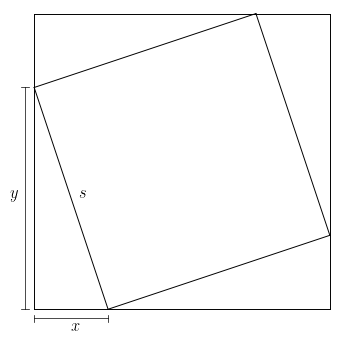
\includegraphics[width=0.45\textwidth]{pics/pythag_proof2.png}
    \caption{Diagram for proof of Pythagoras' theorem.}
    \label{intro:fig:pythag_proof}
\end{figure}


Differential Geometry (DG) is the extension of calculus, linear algebra and multilinear algebra to curved
geometries. Einstein’s Theory of Relativity is written using the language of DG as it is the natural
way to deal with curves, tensor calculus and differential tensor equations in curved spaces. For a basic
introduction to DG, we should start with a manifold $\M$ which is an $N$ dimensional space that locally looks
like $\rspace^N$, $N$ dimensional Euclidean space. This is important as at a point $p\in\M$ we can find infinitesimally
close neighbouring points $p + \delta p \in \M$. In the following sections we will explore curves, functions, tensors and calculus on manifolds using DG.




\subsection{Functions, Curves and Tensors on Manifolds}
A real scalar function $f$ over $\M$ maps any point $p\in \M$ to a real number, denoted 
$f : p \rightarrow \rspace$. An important example of a set of scalar functions is the coordinate system $\phi$, $\phi : p \rightarrow \rspace^N$,
this is normally written $x^\mu$ where $\mu\in\{0,1,...,N-1\}$ is an index labelling the coordinate. The map $\phi$ is called a chart,
and unlike Euclidean space one chart may not be enough to cover the entire manifold; in this case a set
of compatible charts should be smoothly joined, collectively known as an atlas.

Now that functions have been discussed, the next simplest object we can discuss is a curve, or path, through $\M$. A curve $\Gamma$ is a set of smoothly connected points $p(\lambda)\in \M$ that smoothly depend on an input parameter $\lambda \in [\lambda_0,\lambda_1]$. This can be expressed in terms of coordinates as $x^\mu(\lambda)$ where $\phi:p(\lambda) \rightarrow x^\mu(\lambda)$. Differentiating a function $f$ along $\Gamma$ with respect to $\lambda$ gives
\begin{equation} \label{intro:eq:dfdl}
\frac{\dd}{\dd \lambda}f(x^\mu(\lambda)) = \frac{\dd x^\nu}{\dd \lambda}\frac{\partial f(x^\mu)}{\partial x^\nu} = \frac{\dd x^\nu}{\dd \lambda}\partial_\nu f,
\end{equation}
where the Einstein summation convention was invoked, summing over all values of $\nu$, and $\partial_\nu = {\partial}/{\partial x^\nu}$. Equation~(\ref{intro:eq:dfdl}) was derived independantly of the choice of $f$, therefore we can generally write
\begin{equation} \label{intro:eq:ddl}
\frac{\dd}{\dd \lambda} = \frac{\dd x^\nu}{\dd \lambda}\partial_\nu.
\end{equation}
The operator $\dd/\dd \lambda $ can act on any function $f$ and return a new function $\tilde{f}$ over $\M$, this is written as $\dd/\dd \lambda (f) = \tilde{f}$ where $\tilde{f}:p\rightarrow \rspace$ for $p\in\M$. We can also think of $\dd/\dd \lambda$ as a vector $\bs{X}$ with components $X^\mu=\dd x^\mu / \dd \lambda$ and basis vectors $\bs{e}_\mu:=\partial_\mu$ taken from Eq.~(\ref{intro:eq:ddl}). The vector $\bs{X}$ can be written as $\bs{X} = X^\mu \bs{e}_\mu$ and can act on a general function $f$ over $\M$ as $\bs{X}(f) = X^\mu \bs{e}_\mu(f) = X^\mu \partial_\mu f$. Considering the set of all possible curves through a points $p\in\M$, the tangent vector components $\dd x^\mu / \dd \lambda$ span an $N$ dimensional space with basis $\bs{e}_\mu = \partial_\mu$; this space is called the tangent space and is denoted as $\T_p(\M)$ at a point $p\in\M$. 

The next object to discuss is the co-vector which is defined as a map from vectors to real numbers; not to be confused with the dot product in section \ref{intro:sec:dotprod}. Similarly to vectors, a co-vector $\bs{\omega}$ can be expressed as a sum of components $\omega_\mu$ and basis co-vectors $\bs{\theta}^\mu$ like $\bs{\omega} = \omega_\mu \bs{\theta}^\mu$. Contrary to vectors, co-vector components have downstairs indeces and the basis has upstairs indeces; this choice improves the readability of tensor equations when working with components. A co-vector can map a vector to a real number like $\bs{\omega}:\bs{X} \rightarrow \rspace$ or $\bs{\omega}(\bs{X}) \rightarrow \rspace$. Vectors are equally able to map co-vectors to real numbers, denoted as $\bs{X}:\bs{\omega}\rightarrow\rspace$. Co-vectors are defined such that $\bs{\theta}^\mu : \bs{e}_\nu = \delta^\mu_\nu$ where $\delta^\mu_\nu$ are the components of the Kroneka delta equating to zero unless $\mu=\nu$ in which case they are one. The operation of a generic co-vector $\bs{\omega}$ on a generic vector $\bs{X}$ is
\begin{equation}
\bs{\omega}: \bs{X} = \omega_\mu X^\nu \bs{\theta}^\mu:\bs{e}_\nu = \omega_\mu X^\nu \delta^\mu_\nu = \omega_\mu X^\mu \in \rspace.
\end{equation}
This map is linear and identical under reversing the order of operation; $\bs{\omega} : \bs{X} = \bs{X} : \bs{\omega}$. Similarly to vectors, the set of all possible co-vectors at a point $p\in\M$ span an N-dimensional space called the co-tangent space, written as $\T^*_p(\M)$. 

\subsubsection{Multilinear Maps and Tensors}
Generalising the previous linear maps between vectors and co-vectors gives the multilinear map. Consider a tensor $\bs{T}$, this can be expressed in component form like 
\begin{equation}\bs{T} = T^{\alpha\beta, ...}_{\mu\nu,...} \bs{e}_\alpha\otimes\bs{e}_\beta \otimes... \otimes\bs{\theta}^\mu \otimes\bs{\theta}^\nu\otimes...
\end{equation}
for an arbitrary number of outer products of vector and co-vector bases. A tensor with $m$ co-vector bases and $n$ vector bases is called an $(m,n)$ tensor and has a rank of $m+n$. Vectors, co-vectors and scalars are $(1,0)$, $(0,1)$ and $(0,0)$ tensors respectively.  Tensors can act as multilinear maps between tensors. We have already seen how a vector and co-vector can map each other to a scalar, let's extend this with an example. An $(0,2)$ tensor, $\bs{T}=T_{\mu\nu}\bs{\theta}^\mu\otimes\bs{\theta}^\nu$ at $p\in\M$, can map two vectors $\bs{X}$ and $\bs{Y}$ to a scalar as shown, 
\begin{align}
\bs{T}(\bs{X},\bs{Y}) 
&=T_{\mu\nu}X^\alpha Y^\beta \bs{\theta}^\mu \otimes \bs{\theta}^\nu (\bs{e}_\alpha,\bs{e}_\beta),\\
&= T_{\mu\nu}X^\alpha Y^\beta (\bs{\theta}^\mu:\bs{e}_\alpha)( \bs{\theta}^\nu:\bs{e}_\beta) ,\\
&= T_{\mu\nu}X^\alpha Y^\beta \delta^\mu_\alpha  \delta^\nu_\beta ,\\
&= T_{\mu\nu}X^\mu Y^\nu.
\end{align}
The multilinear map can also output generic tensors, for example consider 
\begin{equation}
\bs{T}(\bs{X},\star) = T_{\mu\nu} X^\alpha (\bs{\theta}^\mu:\bs{e}_\alpha)\bs{\theta}^\nu = T_{\mu\nu}X^\mu \bs{\theta}^\nu,
\end{equation}
which uses the $(0,2)$ tensor $\bs{T}$ to map the vector $\bs{X}$ to a co-vector $\bs{W}$ with components $W_\mu = T_{\mu\nu}X^\mu$.

One final example of a mapping is from a single tensor to a lower rank tensor, this is called contraction. To illustrate this, let's take a $(1,3)$ tensor $\bs{Z} = Z^\alpha_{\,\,\,\mu\nu\rho} \bs{e}_\alpha \otimes\bs{\theta}^\mu\otimes\bs{\theta}^\nu\otimes\bs{\theta}^\rho$. We can choose to use the basis vector $\bs{e}_\alpha$ to act on any of the three co-vector bases, choosing $\bs{\theta}^\mu$ this is
\begin{equation}
Z^\alpha_{\,\,\,\mu\nu\rho} (\bs{e}_\alpha : \bs{\theta}^\mu)\bs{\theta}^\nu\otimes\bs{\theta}^\rho = Z^\mu_{\,\,\,\mu\nu\rho}\bs{\theta}^\nu\otimes\bs{\theta}^\rho = \tilde{Z}_{\nu\rho}\bs{\theta}^\nu\otimes\bs{\theta}^\rho,
\end{equation} 
where $\tilde{Z}_{\nu\rho} = Z^\mu_{\,\,\,\mu\nu\rho}$.





\subsection{The Inner Product and the Metric} \label{intro:sec:dotprod}
To introduce the notion of length on a tanget plane $\T_p(\M)$ at a point $p\in\M$ the metric tensor $\bs{g}$ is introduced. The metric tensor has componenets, 
\begin{equation}
g_{\mu\nu} = \bs{e}_\mu \cdot \bs{e}_\nu,
\end{equation}
where $\bs{e}_\mu \cdot \bs{e}_\nu$ represents the inner product (or dot product) on $\T_p(\M)$; clearly the metric is symmetric by construction as $\bs{e}_\mu \cdot \bs{e}_\nu=\bs{e}_\nu \cdot \bs{e}_\mu$. The inner product can be thought of as a multilinear map,
\begin{gather}
\bs{g} : (\bs{X} , \bs{Y}) \rightarrow \rspace , \quad \mathrm{or} \quad
\bs{g}(\bs{X},\bs{Y}) = g_{\mu\nu} X^\mu Y^\nu,
\end{gather}
where $\bs{X}\in \T_p(\M)$, $\bs{Y}\in \T_p(\M)$ and $\bs{g}\in \T^*_p(\M)\otimes  \T^*_p(\M)$. The inner product can also be represented by a second map
\begin{gather}
\bs{X} : \bs{Y} \rightarrow \rspace , \quad \mathrm{or} \quad
\bs{X} \cdot \bs{Y} = X^\mu Y^\nu \bs{e}_\mu \cdot \bs{e}_\nu = X^\mu Y^\nu g_{\mu\nu},
\end{gather}
which is a new mapping. The inner product also gives the length $|\bs{X}|$ or magnitude of any vector $\bs{X}\in \T_p(\M)$ as,
\begin{equation}
|\bs{X}|^2 = \bs{X} \cdot \bs{X} = g_{\mu\nu}X^\mu X^\nu.
\end{equation}
Another way to think of the inner product is that the metric maps a vector $\bs{X}$ to an equivalent or {\it dual} co-vector $\bs{\Xi}$ such that $\bs{X} : \bs{\Xi} = X^\mu \Xi_\mu= g_{\mu\nu}X^\mu X^\nu$. In component form $\bs{\Xi}$ is
\begin{align}
\Xi_\mu = g_{\mu\nu}X^\nu;
\end{align}
this use of the metric to map a vector to it's corresponding co-vector (and vica versa) is extremely useful. Without loss of information we can write $\Xi_\nu = X_\nu$ to make it obvious that $X_\nu = X^\mu g_{\mu\nu}$ and this convention will be used from now on.

The metric also assigns an inner product and a length measure on the co-tangent plane $\T^*_p(\M)$ but instead using the inverse components $g^{\mu\nu} = (g^{-1})_{\mu\nu}$,
\begin{equation}
g^{\mu\nu} = \bs{\theta}^\mu \cdot \bs{\theta}^\nu.
\end{equation}
Similarly to before the inner product of two co-vectors $\bs{\omega}$ and $\bs{\sigma}$ is
\begin{equation}
\bs{\omega} \cdot \bs{Y} = \omega_\mu \sigma_\nu \bs{\theta}^\mu \cdot \bs{\theta}^\nu = \omega_\mu \sigma_\nu g^{\mu\nu} = \omega_\mu \sigma^\mu.
\end{equation}
The reason that $g^{\mu\nu}$ must be the inverse matrix to $g_{\mu\nu}$ is as follows. For a vector $X^\mu \bs{e}_\mu$ and a co-vector $\omega_\mu \bs{\theta}^\mu$ we would like, 
\begin{align}
\bs{X} : \bs{\omega} &= \bs{g}(\bs{X},\star) : \bs{g}^{-1}(\bs{\omega},\star) ,\\
X^\mu \omega_\mu  &= X_\mu \omega^\mu ,\\
&= X^\rho g_{\rho\mu}g^{\mu\sigma} \omega_\sigma
\end{align}
which is only true if $g_{\rho\mu}g^{\mu\sigma} = \delta^\sigma_\rho$ which is true by definition if $(g^{-1})_{\mu\nu} = g^{\mu\nu}$.

Not only has the metric provided us with an inner product and a length on tangent planes and cotangent planes, but it has also given a mapping between the two and can raise and lower indeces on general tensors such as
\begin{equation}
T^{\mu\nu ...}_{\,\,\,\,\,\, \alpha \beta} = g^{\mu\rho}g_{\beta\sigma}T^{\,\,\, \nu \,\,\, \sigma ....}_{\rho \,\,\, \alpha}.
\end{equation}



\subsection{Maps Between Manifolds}\label{intro:sect:map}
In section we will be interested in the maps between two manifolds $M$ and $N$. This has many uses such as pushing and pulling tensors between manifolds, allowing us to calculate a Lie derivative of tensor fields and finding the metric (or any tensor field) on an embedded surface; this very importantly allowed us to perform the 3+1 decomposition on a spacetime as in section \ref{nr:sec:3plus1}.

Define a smooth map $\Phi : M \rightarrow N$ between manifolds on some coordinate patch labelling coordinates $x^\mu\in M$ and $y^\mu\in N$. The map $\Phi:x^\mu \rightarrow y^\mu$ gives $y^\mu = \Phi^\mu(x^\nu)$, or equivalently $y^\mu(x^\nu)$. Scalar functions must also map trivially $f_N(y^\mu(x^\nu))=f_M(x^\mu)$ where $f_N\in N$ and $f_M \in M$, thus we will no longer identify which manifold a function is on. The map $\Phi$ allows us to push the vector $\bs{X}\in\T_p(M)$ to $\Phi_* \bs{X} \in \T_q(N)$, where $q=\Phi(p)$, in a way such that it's action on a function $f$ is the same in either manifold. 
\begin{align}
\bs{X}(f)\Big|_p &= \Phi_*\bs{X}(f)\Big|_q ,\\
X^\mu \frac{\partial f}{\partial x^\mu}  &= (\Phi_* X)^\nu\frac{\partial f}{\partial y^\nu} , \\
\left( X^\mu \frac{\partial y^\nu}{\partial x^\mu}\right) \frac{\partial f}{\partial y^\nu}  &= (\Phi_* X)^\nu\frac{\partial f}{\partial y^\nu},
\end{align} 
and hence the components of the push-foreward $\Phi_* \bs{X}$ can be read off,
\begin{equation}
(\Phi_* X)^\mu = \frac{\partial y^\mu}{\partial x^\nu}X^\nu.
\end{equation}
Given a co-vector field $\bs{\omega} \in \T^*_p(N)$ we can pull the field back from $\T^*_p(M) \leftarrow \T^*_q(N)$, denoted $\Phi^*\bs{\omega}$, by demanding that $\Phi^*\bs{\omega}(\bs{X})\big|_p = \bs{\omega}(\Phi_* \bs{X})\big|_q$. Evaluating this gives 
\begin{align}
\Phi^*\bs{\omega}(\bs{X})\Big|_p &= \bs{\omega}(\Phi_* \bs{X})\Big|_q, \\
(\Phi^* \omega)_\mu X^\mu&= \omega_\nu (\Phi_*X)^\nu , \\ 
(\Phi^* \omega)_\mu X^\mu&= \omega_\nu \frac{\partial y^\nu}{\partial x^\mu} X^\mu ,
\end{align}
and the components of the pull-back $\Phi_*\bs{\omega}$ can be read off,
\begin{align}
(\Phi^* \omega)_\mu &= \omega_\nu \frac{\partial y^\nu}{\partial x^\mu}.
\end{align}
Considering an $(0,2)$ tensor $\bs{T} \in N$, the pullback $\Phi^*\bs{T} \in M$ follows simply from demanding that $\bs{T}(\Phi_* \bs{X},\Phi_*\bs{Y})|_q = \Phi^*\bs{T}(\bs{X},\bs{Y})|_p$ where $\bs{X}$ and $\bs{Y}$ are vector fields on $M$. The components of the pull-back of $\bs{T}$ are therefore
\begin{equation}
(\Phi^*T)_{\mu\nu} = \frac{\partial y^\rho}{\partial x^\mu} \frac{\partial y^\sigma}{\partial x^\nu}T_{\rho\sigma}.
\end{equation}
The pull-back of a generic $(0,q)$ tensor and the push-foreward of a generic $(p,0)$ tensor can be found similarly by contracting with an extra $\frac{\partial y^\mu}{\partial x^\nu}$ for each downstairs index or $\frac{\partial x^\mu}{\partial y^\nu}$ for each upstairs index.


\subsubsection{Diffeomorphisms}
So far we have only discussed the one way mapping $\Phi :M \rightarrow N$ which is requires a well behaved $\partial y^\nu / \partial x^\mu$. A diffeomorphism is an isomorphism\footnote{An isomorphism is a structure preserving bijective map between sets.} between smooth manifolds $\Phi :M \rightarrow N$, meaning $M$ and $N$ have the same number of dimensions. Two infinitessimally close points $\{p,p+\delta p\}\in\M$ map to two infinitessimally close points $(q,q+\delta q)\in\mathcal{N}$ meaning that open sets are preserved. Given that a diffeomorphism is smooth bijective map then it must be invertible with inverse map $\Phi^{-1}:N \rightarrow M$, and $y^\nu(x^\mu)$ has a smooth inverse $x^\nu(y^\mu)$. When an inverse map $\Phi^{-1}$ is defined then the pull-back of $(p,0)$ tensors from $N$ to $M$ along with the push-foreward of $(0,q)$ tensors from $M$ to $N$ is possible. This means it is possible to push or pull generic tensors between $M$ and $N$ in any direction. The tangent spaces associated with $p \in \M$ or $q \in \mathcal{N}$ are therefore also preserved under mapping meaning that local structure on the manifold is preserved under the mapping. Two common examples of diffeomorphisms are coordinate changes and translations.

\subsubsection{Projection Mappings}
As mentioned, maps between manifolds can be used to project tensors to lower dimensional embedded surfaces. This requires us to consider an $m$ dimensional manifold $M$ with metric $g_{\mu\nu}$ and coordinates $x^\mu$ aswell as an embedded $n$ dimensional surface $N$ where $n<m$. We can treat $N$ as a separate $n$ dimensional manifold with metric $h_{\mu\nu}$. As before, we can define a map $\Phi:x^\mu \rightarrow y^\mu$ and the pullback of the metric demands that,
\begin{equation}
{}^{(m)}h_{\rho\sigma} = {}^{(n)}h_{\mu\nu}\frac{\partial y^\mu  }{\partial x^\rho  } \frac{\partial y^\nu  }{\partial x^\sigma  },
\end{equation}
where ${}^{(m)}\bs{h}$ represents m-dimensional the tensor on $M$ and ${}^{(n)}\bs{h}$ represents n-dimensional the tensor on $N$; of course ${}^{(n)}\bs{h}$ and $\bs{h}$ are completely identical.

In the case that $n=m-1$, which is a projection into one less dimension, a convenient form for ${}^{(n)}\bs{h}$ can be found. If the image of $N$ in $M$ has everywhere an m-dimensional unit normal $\bs{n}$, then a vector $\bs{X}\in \T_p(\M)$ for $p\in N$ can be projected onto $N$ like,
\begin{equation}
({}^{(m)}\overrightarrow{{X}})^\mu = (\delta^\mu_\nu \mp n^\mu n_\nu )X^\nu,
\end{equation}
where the sign is negative if $|\bs{n}|^2=1$ and positive if $|\bs{n}|^2 = -1$. It should be noted that strictly, $\overrightarrow{\bs{X}} \in \T_p(\M)$. To avoid confusion we will denote the m-dimensional projected vector as ${}^{(m)}\overrightarrow{\bs{X}}$ and vector existing in the n-dimensional manifold $N$ as ${}^{(n)}\overrightarrow{\bs{X}}$. The projection guarentees that,
\begin{align}
{}^{(n)}\bs{h} ({}^{(n)}\overrightarrow{\bs{X}},{}^{(n)}\overrightarrow{\bs{X}}  ) &= \bs{g} ({}^{(m)}\overrightarrow{\bs{X}},{}^{(m)}\overrightarrow{\bs{X}}  ),\\
&= {}^{(m)}{h}_{\mu\nu} (\delta^\mu_\alpha \mp n^\mu n_\alpha) {{X}}^\alpha(\delta^\nu_\beta \mp n^\nu n_\beta) {{X}}^\beta  ,\\
&= {}^{(m)}\bs{h} ({\bs{X}},{\bs{X}}  ),
\end{align}
which gives a formula for the projected metric ${}^{(m)}\bs{h} \in \M$,
\begin{equation}
{}^{(m)}h_{\mu\nu} = g_{\mu\nu} \mp n_\mu n_\nu.
\end{equation}
The use of this projected metric to project general tensors to lower dimensions is explored in detail in section \ref{nr:sec:3plus1}. 


Mapping to lower dimensional surface of $d$ dimensions can be done similarly by adding an extra mutually-orthogonal unit vector for each reduced dimension like,
\begin{equation}
{}^{(d)}h_{\mu\nu} = g_{\mu\nu} \mp n^{(1)}_\mu n^{(1)}_\nu  \mp n^{(2)}_\mu n^{(2)}_\nu + ... \,\,.
\end{equation}

The metric $\bs{h}$ on an arbitrary a-dimensional sub-surface $A\in\M$ can be explicitly calculated from the pushforeward of ${}^{(m)}\bs{h}$ considering the diffeomorphism $\Phi^A$ that maps the image of $A$ embedded in $\mathcal{M}$ to an a-dimensional manifold $\mathcal{A}$. The resulting metric is, 
\begin{equation}
(\Phi^A_* g)_{ij} = h_{ij} = \frac{\partial x^\mu}{\partial z^i} \frac{\partial x^\nu}{\partial z^j} {}^{(m)}h_{\mu\nu}  = \frac{\partial x^\mu}{\partial z^i} \frac{\partial x^\nu}{\partial z^j}\left( g_{\mu\nu}\mp n^{(1)}_\mu n^{(1)}_\nu  \mp n^{(2)}_\mu n^{(2)}_\nu + ...  \right), \label{intro:eq:projectedmetric}
\end{equation}
where $n^{(i)}$ are a set of orthogonal unit vectors perpendicular to $A$; $x^\mu$ span $\M$ and $z^i$ span $\mathcal{A}$.



\subsection{Lie Derivatives}\label{intro:sec:lie_deriv}

The Lie derivative of a tensor at a point $p$ is the rate of change of a tensor field with respect to a pull-back from a diffeomorphism $\Phi$ mapping infinitessimally close points $p=x^\mu,q= x^\mu+\epsilon \xi^\mu \in \mathcal{M}$ like $\Phi:p \rightarrow q $ for some vector field $\bs{\xi}$. Like any good differential operator, the Lie deriviative $\L_\xi$ along $\bs{\xi}$ (and $\L_\zeta$ along vector field $\bs{\zeta}$) should obey,
\begin{align}
\L_{a \xi + b \zeta}\bs{T}  &= a \L_\xi\bs{T}  + b \L_\zeta\bs{T} ,\\
\L_\xi (a \bs{T} + b \bs{W}) & = a \L_\xi \bs{T} + b \L_\xi \bs{W} , \\
\L_\xi (f \bs{T} ) &= \bs{T} \L_\xi f + f \L_\xi \bs{T} \label{intro:eq:lie_liebnitz},
\end{align}
for constant $\{a,b\}$, function $f$ and generic tensorial objects of same type $\bs{T}$ and $\bs{W}$. 

The simplest example is the Lie derivative of a scalar field $\phi$, denoted $\L_\xi \phi$ with respect to vector field $\bs \xi$,
\begin{align} \label{intro:eq:Lxiphi}
\L_\xi \phi &= \lim_{\epsilon \rightarrow 0}\left[\frac{\Phi^*\phi\vert_q - \phi\vert_p}{\epsilon} \right] , \\
&= \lim_{\epsilon \rightarrow 0}\left[\frac{\phi(x^\mu + \epsilon \xi^\mu) - \phi(x^\mu)}{\epsilon} \right] , \\
&= \xi^\mu \partial_\mu \phi,
\end{align}
which reduces to the partial derivative of $\phi$ with along $\bs{\xi}$. Next let's calculate the Lie derivative of a vector field $\bs{X}$ with respect to vector field $\bs\xi$. Starting with the same definition as Eq.~(\ref{intro:eq:Lxiphi}), and using $y^\mu = x^\mu + \epsilon \xi^\mu$, the Lie derivative of $\bs X$ is, 
\begin{align} 
(\L_\xi {X})^\mu &= \lim_{\epsilon \rightarrow 0}\left[\frac{(\Phi^*X\vert_q)^\mu - {X\vert_p}^\mu}{\epsilon} \right] , \\
&= \lim_{\epsilon \rightarrow 0}\left[\frac{ \frac{\partial x^\mu}{\partial y^\nu}X^\nu(x^\rho + \epsilon \xi^\rho) - X^\mu(x^\rho)}{\epsilon} \right] , \\
&= \lim_{\epsilon \rightarrow 0}\left[\frac{ (\delta_\nu^\mu - \epsilon \partial_\nu \xi^\mu)X^\nu(x^\rho + \epsilon \xi^\rho) - X^\mu(x^\rho)}{\epsilon} \right] , \\
&= \lim_{\epsilon \rightarrow 0}\left[\frac{ - \epsilon \partial_\nu \xi^\mu X^\nu(x^\rho + \epsilon \xi^\rho)+ X^\mu(x^\rho + \epsilon \xi^\rho) - X^\mu(x^\rho)}{\epsilon}  \right] , \\
&= \lim_{\epsilon \rightarrow 0}\left[\frac{ - \epsilon \partial_\nu \xi^\mu X^\nu(x^\rho)+ X^\mu(x^\rho + \epsilon \xi^\rho) - X^\mu(x^\rho)+\mathcal{O}(\epsilon^2)}{\epsilon}  \right] , \\
&= \xi^\nu \partial_\nu X^\mu - X^\nu \partial_\nu \xi^\mu.
\end{align}
The Lie derivative for co-vectors and tensors can be derived in the same way, but can be quickly derived from the Liebnitz rule as follows. Define a scalar field $\psi$, vector field $\bs{X}$ and co-vector field $\bs\omega$, where $\psi = X^\mu \omega_\mu$, then it follows that,
\begin{align}
\L_\xi \psi &= \xi^\mu \partial_\mu \psi =  X^\nu\xi^\mu\partial_\mu\omega_\nu+\omega_\nu\xi^\mu\partial_\mu X^\nu, \\
              &= \L_\xi (X^\mu \omega_\mu),\\
              &= \omega_\mu (\L_\xi X)^\mu + X^\mu(\L_\xi\omega)_\mu,\\
               X^\mu(\L_\xi \omega)_\mu & =X^\nu\xi^\mu\partial_\mu\omega_\nu+\omega_\nu\xi^\mu\partial_\mu X^\nu-\omega_\mu (\L_\xi X)^\mu, \\
               (\L_\xi \omega)_\mu&= \xi^\nu \partial_\nu \omega_\mu + \omega_\nu \partial_\mu \xi^\nu.
\end{align}
Derivatives of a generic tensor $\bs{T}$ follows simply, for example,
\begin{equation}(\L_\xi T )^{\alpha\beta ...}_{\,\,\,\,\,\,\mu\nu...} = \xi^\sigma \partial_\sigma T^{\alpha\beta ...}_{\,\,\,\,\,\,\mu\nu...} + T^{\alpha\beta ...}_{\,\,\,\,\,\,\sigma\nu...} \partial_\mu \xi^\sigma + T^{\alpha\beta ...}_{\,\,\,\,\,\,\mu\sigma...} \partial_\nu \xi^\sigma + ... - T^{\sigma\beta ...}_{\,\,\,\,\,\,\mu\nu...}\partial_\sigma \xi^\alpha - T^{\alpha\sigma ...}_{\,\,\,\,\,\,\mu\nu...}\partial_\sigma \xi^\beta - ...\,.
\end{equation} 





\subsection{Lengths on Manifolds}\label{intro:sect:lgm}
The natural entry point for studying curved geometry is to revisit Pythagoras' theorem. For this we need a manifold $\M$ equipped with a metric $\bs{g}$, written as $(\M,\bs{g})$ for short. The distance $\dd s$ between two infinitessimaly close points $p\in\M$ and $p+\delta p \in \M$, with coordinates $p=x^\mu$ and $p+\delta p = x^\mu + \dd x^\mu$, is given by
\begin{equation}
\dd s^2 = \bs{g}(\bs{\mathrm{d}}\bs{x},\bs{\mathrm{d}}\bs{x}) =  g_{\mu\nu}\dd x^\mu \dd x^\nu,
\end{equation}
where $g_{\mu\nu}$ are the components of the metric tensor. This is the generalisation of Eq.~(\ref{intro:eq:pythag_inf}) to curved space; noteably the line element can now have varying coefficients from $g_{\mu\nu}$ and cross terms such as $\dd x \dd y$. The special choice of $g_{\mu\nu} = \delta_{\mu\nu}$ gives us flat space, also called Euclidean space, where $\delta_{\mu\nu}=1$ if $\mu=\nu$ and vanishes otherwise. With the line elemend defined, we can immediately apply it to calculating the length of a general curve in curved space. Consider the curve $\Gamma$ consisting of a set of connected points $p(\lambda)\in\M$ smoothly parameterised by $\lambda$. We can calculate the length $\Delta s$ of the curve between $\lambda_1 \geq\lambda\geq\lambda_0$ by parameterising $\dd s$,
\begin{equation}
\dd s ^2 = g_{\mu\nu}\frac{\partial x^\mu}{\partial \lambda}\frac{\partial x^\nu}{\partial \lambda}\dd \lambda^2,
\end{equation}
and integrating $\dd s$ along $\Gamma$,
\begin{equation}
\label{intro:eq:Delta_s}\Delta s = \int_{\lambda_0}^{\lambda_1}\sqrt{\left(g_{\mu\nu}\frac{\partial x^\mu}{\partial \lambda}\frac{\partial x^\nu}{\partial \lambda}\right)}\dd \lambda.
\end{equation}
In the simplified case where $\lambda$ is one of the coordinates, say $\xi$, the length $\Delta s$ becomes,
\begin{align} \label{intro:eq:coord_interval_length}
\Delta s &= \int_{\xi_0}^{\xi_1}\sqrt{g_{\xi\xi}}\dd \xi.
\end{align}




\subsection{Volumes on Manifolds}

Following from measuring the length of a curve now we can measure volumes on a manifold; of course we still require a metric $\bs{g}$ over the manifold. Let's say that in a coordinate system $x^\mu$ we can define the volume $V$ of a subregion $M$ by integrating some weight function $w(x^\mu)$,
\begin{equation}
V = \int_{M} w(x^\mu) \dd x^1 \dd x^2 ... \dd x^n,
\end{equation}
over $M$. To find $w(x^\mu)$, start by defining an orthogonal coordinate transformation $x^\mu \rightarrow \tilde{x}^\mu$ such that $\tilde{\bs{g}}$ is diagonal and $\det(\bs{g})=\det(\tilde{\bs{g}})$; this is always possible as $\bs{g}$ is real and symmetric. In this coordinate system, the volume $\delta V$ in an infinitessimal cuboid, with $i$'th sidelength $\delta \tilde{x}^i$, is
\begin{align}
\delta V &=  \left( \sqrt{\tilde{g}_{11}}\delta \tilde{x}^1 \right)\left(\sqrt{\tilde{g}_{22}}\delta \tilde{x}^2 \right)... \left(\sqrt{\tilde{g}_{nn}}\delta \tilde{x}^n\right) , 
\end{align}
where Eq.~(\ref{intro:eq:coord_interval_length}) was used to get the length bewteen each $\tilde{x}^i$ and $\tilde{x}^i + \delta \tilde{x}^i$. Given that $\tilde{\bs{g}}$ is diagonal we know the $i$'th eigenvalue $\tilde{\lambda}_i = \tilde{g}_{ii}$ and therefore $\det(\tilde{\bs{g}})$ = $\prod_i \tilde{g}_{ii}$. Thus the volume $\delta V$ can be rewritten,
\begin{align}
\delta V &=  \sqrt{|\det(\tilde{\bs{g}})|}\delta \tilde{x}^1 \delta \tilde{x}^2  ... \delta \tilde{x}^n , 
\end{align} 
and the formula for the finite volume of $M$ is,
\begin{equation} \label{intro:eq:volume_curved}
V = \int_{M} \sqrt{|\det(\tilde{\bs{g}})|} \dd \tilde{x}^1 \dd \tilde{x}^2 ... \dd \tilde{x}^n,
\end{equation}
and the form of the weight function in $\tilde{x}^\mu$ coordinates is $\tilde{w}(\tilde{x}^\mu)= \sqrt{|\det(\tilde{\bs{g}})|}$.
We are now free to transform back from $\tilde{x}^\mu\rightarrow x^\mu$, and given that the transformation is orthogonal we know that $\det(\bs{g})=\det(\tilde{\bs{g}})$ and the Jacobean matrix $\bs{J}$ of the coordinate transformation has $\det({\bs{J}})=1$, therefore
\begin{equation}\label{intro:eq:volume_curved2}
V = \int_{M} \sqrt{|\det({\bs{g}})|} \dd {x}^1 \dd {x}^2 ... \dd {x}^n,
\end{equation}
which holds for any non-diagonal, real and symmetric metric $\bs{g}$. In general we will now denote the deteminant of a metric $\det(\bs{g})$ with the lower case letter $g$. When dealing with a pseudo-Riemannian manifold with a negative determinant, such as spacetime, it is more common to see $\sqrt{-g}$ written rather than $\sqrt{|g|}$ giving
\begin{equation}
V = \int_{M}\sqrt{-g} \,\dd {x}^1 \dd {x}^2 ... \dd {x}^n.
\end{equation}
Equation~(\ref{intro:eq:volume_curved2}) can also be used to find the volume (or area) of a lower dimensional sub-volume. First cover the new sub-volume $A$ with coordinates $z^\mu$, where $\mu\in\{1,2,...,m\}$ for $m<n$, and then calculate the metric $\bs{h}$ which can be done using Eq.~(\ref{intro:eq:projectedmetric}). The area $V_A$ of $A$ is then, 
\begin{equation} \label{intro:eq:area_int}
V_A = \int_{A}\sqrt{|h|} \,\dd {z}^1 \dd {z}^2 ... \dd {z}^m,
\end{equation}
which can be seen by mapping to an a-dimensional manifold $\mathcal{A}$ that is diffeomorphic to $A$ and applying Eq.~(\ref{intro:eq:volume_curved2}).



 \subsection{Geodesics} \label{intro:sec:geodesics}


 For a manifold equipped with metric $(\M,g)$ the curve with shortest distance between two points $p,q\in\M$ is called a geodesic. To find the geodesic joining $p$ and $q$ we need to use calculus of variation on the total length $\Delta s$ from Eq.~(\ref{intro:eq:Delta_s}) of a general curve between two points. Given that the integrand $\L$ of Eq.~(\ref{intro:eq:Delta_s}) is a function like $\L(x^\mu,\dot{x}^\mu)$, where the dot means differentiation by $\lambda$, we can use the Eular-Lagrange equation,
\begin{align}
\frac{\partial{\L}}{\partial x^\mu} - \frac{\dd}{\dd \lambda}\frac{\partial \L}{\partial \dot{x}^\mu} = 0,
\end{align}
to give a differential equation with solution being a geodesic. Applyin the EL equation to the integrand of Eq.~(\ref{intro:eq:Delta_s}) is algebraically messy, it is easier\footnote{Given that $\L$ is homogeneneus to degree k, $\dot{x}^i \partial \L / \partial \dot{x}^i = k\L$ for constant k, one can show that $\dd\L/\dd\lambda=0$ if the Eular-Lagrange equation is assumed.} to square the integrand and start from $\L^2$ giving the same solution if $\dd \L / \dd \lambda=0$, 
\begin{align}
\frac{\partial{\L^2}}{\partial x^\alpha} &- \frac{\dd}{\dd \lambda}\frac{\partial \L^2}{\partial \dot{x}^\alpha} = 0, \\
\frac{\partial}{\partial x^\alpha} \left(g_{\mu\nu}\dot{x}^\mu\dot{x}^\nu\right) &- \frac{\dd}{\dd \lambda}\frac{\partial }{\partial \dot{x}^\alpha}\left(g_{\mu\nu}\dot{x}^\mu\dot{x}^\nu\right) = 0, \\
(\partial_\alpha g_{\mu\nu})\dot{x}^\mu\dot{x}^\nu &- 2\frac{\dd}{\dd \lambda}\left(g_{\alpha\nu}\dot{x}^\nu\right) = 0, \\
(\partial_\alpha g_{\mu\nu})\dot{x}^\mu\dot{x}^\nu &- 2\left(\dot{x}^\rho \partial_\rho \left(g_{\alpha\nu}\right)\dot{x}^\nu\right) - 2\ddot{x}^\nu g_{\alpha\nu} =0. 
\end{align}
Rearranging and multiplying by $g^{\alpha\beta}$ gives,
\begin{align}
\ddot{x}^\beta &+ \frac{1}{2}g^{\alpha\beta}\left(\partial_{\mu}g_{\alpha\nu} +\partial_{\nu}g_{\alpha\mu} -\partial_{\alpha}g_{\mu\nu} \right)\dot{x}^\mu\dot{x}^\nu=0,\\
 \ddot{x}^\beta &+ \Gamma^\beta_{\,\,\,\mu\nu}\dot{x}^\mu\dot{x}^\nu=0, \label{intro:eq:geodesic}
\end{align}
where $\Gamma^\beta_{\,\,\,\mu\nu}$ is the components of the connection-symbol from Eq.~(\ref{intro:eq:christoffel_def}). A trivial solution to Eq.~(\ref{intro:eq:geodesic}) is in flat space using cartesian coordinates where $\Gamma^\beta_{\,\,\,\mu\nu}=0$ and therefore $\ddot{x}^\beta=0$ so $\dot{x}^\beta$ is a constant; this tells us the shortest distance between two points in flat space is a straight line. In other words, geodesics are straight lines in flat space.


\subsubsection*{Non-affine Geodesics}
The equation of a geodesic given above is true for an affinely parameterised curve. An affine parameter $\lambda$ is defined so that the length of a curve $\delta s$ between two parameter values $\lambda$ and $\lambda+\delta \lambda$ is given by $\delta s = k (\delta \lambda)$ for constant $k$; the arclength along a curve is linearly proportional to the value of the $\lambda$. This property was inherant in the derivation of Eq.~(\ref{intro:eq:geodesic}) is that $\dd \L / \dd \lambda=0$ was assumed.

A non-affine parameter $\mu$ could equally be used to describe the curve. Writing $\mu(\lambda)$ the geodesic equation is transformed as shown,
\begin{align}
\frac{\dd ^2 {x}^\beta}{\dd \lambda^2} &+ \Gamma^\beta_{\,\,\,\mu\nu}\frac{\dd {x}^\mu}{\dd \lambda}\frac{\dd {x}^\nu}{\dd \lambda}=0,\\
\left(  \frac{\dd^2 \mu}{\dd \lambda^2} \frac{\dd}{\dd\mu}  + \left( \frac{\dd \mu}{\dd \lambda} \right)^2 \frac{\dd^2}{\dd \mu^2} \right) {x}^\beta     &+ \Gamma^\beta_{\,\,\,\mu\nu}\frac{\dd {x}^\mu}{\dd \mu}\frac{\dd {x}^\nu}{\dd \mu}\left( \frac{\dd \mu}{\dd \lambda} \right)^2=0,\\
    \frac{\dd^2 {x}^\beta }{\dd \mu^2}     &+ \Gamma^\beta_{\,\,\,\mu\nu}\frac{\dd {x}^\mu}{\dd \mu}\frac{\dd {x}^\nu}{\dd \mu}=- \left( \frac{\dd \mu}{\dd \lambda} \right)^{-2}\frac{\dd^2\mu}{\dd \lambda^2} \frac{\dd x^\beta}{\dd\mu},\\
    \frac{\dd^2 {x}^\beta }{\dd \mu^2}     &+ \Gamma^\beta_{\,\,\,\mu\nu}\frac{\dd {x}^\mu}{\dd \mu}\frac{\dd {x}^\nu}{\dd \mu}=- f(\mu) \frac{\dd x^\beta}{\dd\mu},\\
\end{align}
which is the same as the affine geodesic equation except with an extra non-zero right hand side proportional to $\dd x^\beta/\dd \mu$ and some function $f(\mu)$. If $\mu$ is a linear function of $\lambda$ then $\mu$ is also an affine parameter; this is reflected in the term $\dd^2 \mu / \dd \lambda^2=0$ and the affine geodesic equation is returned.


MAYBE IM BETTER OFF DERIVING THE GEODESIC EQUTION FROM L NOT L SQAURED WHICH GIVES
\begin{equation}
\frac{1}{\mathcal{L}}\left(  \dot{x}^\mu \dot{x}^\nu \partial_\alpha g_{\mu\nu} - 2\dot{x}^\mu \frac{\dd}{\dd \lambda}g_{\mu\alpha} - 2 g_{\mu\alpha}\ddot{x}^\mu+ \underbrace{\frac{2}{\mathcal{L}}g_{\mu\nu}\dot{x}^\mu \frac{\dd\mathcal{L}}{\dd \lambda}}_{{this\,\, is\,\, the\,\, non-affine\,\, bit}}\right)=0
\end{equation}


\section{Tensor Calculus and Curvature}


\subsection{General Covariance and Coordinate transformations}\label{intro:sec:cov}
Many laws of physics can be expressed as tensor field equations where a tensor field is the assignment of a tensor to each point in space. This assignment must be smooth as it is to describe physical quantities. The power of tensor algebra and tensor calculus is that if a tensor field equation can be written in one coordiante system then must hold (in index form) in all sensible coordinate system. This is a consequence of the tensor transformation law. Looking back, we can write a generic vector $\bs{X}$ as $X^\mu \bs{e}_\mu = X^\mu \partial_\mu$ and if we choose a coordinate transformation $x^\mu \rightarrow \tilde{x}^\mu$ then we see that in the transformed coordinate system the vector field $\bs{X}$, written $\tilde{\bs{X}}$, becomes
\begin{align}
\tilde{\bs X} &= \tilde{X}^\mu\frac{\partial}{\partial \tilde{x}^\mu}, \\
              &= \tilde{X}^\mu\frac{\partial x^\nu}{\partial \tilde{x}^\mu}\frac{\partial}{\partial {x}^\nu}, \\
              &= X^\nu \frac{\partial}{\partial x^\nu}, \\
              &= \bs{X}, \
\end{align}
where the components $X^\nu = \tilde{X}^\mu\frac{\partial x^\nu}{\partial \tilde{x}^\mu}$ are required to transform in order to ensure $\bs{X}=\tilde{\bs{X}}$. This says that the underlying geometric object (a vector in this case) is independant of the coordinates used to describe them; the tradeoff for this useful property is that the vectors components $X^\mu$ have to transform under the tensor transformation law, effectively opposing the transformation of the basis vectors. Working from a co-vector $\omega$ we can write it as $\omega_\mu \bs{\theta}^\mu = \omega_\mu \dd x^\mu$ in component-basis form [REF THIS?] and the same coordinate transform gives
\begin{align}
\tilde{\bs{\omega}} &= \tilde{\omega}_\mu \dd \tilde{x}^\mu , \\
                    &= \tilde{\omega}_\mu \frac{\partial \tilde{x}^\mu}{\partial x^\nu}\dd {x}^\nu , \\
                    &= \omega_\nu \dd x^\nu,
\end{align}
where the co-vector components transform like $\omega_\nu= \tilde{\omega}_\mu \frac{\partial \tilde{x}^\mu}{\partial x^\nu}$, the opposite way to the vector components. These transformation laws ensure that a scalar field created from the product of a vector field and a co-vector field, like $\bs{\omega}:\bs{X}$, is a Lorentz scalar not transforming under coordinate transformations. This can be seen from
\begin{align}
\tilde{\bs \omega} : \tilde{\bs X} &= \tilde{X}^\mu \tilde{\omega}_\mu ,\\
                                   &= {X}^\nu \frac{\partial \tilde{x}^\mu}{\partial x^\nu}   \frac{\partial x^\rho}{\partial \tilde{x}^\mu}\omega_\rho, \\
                                   &=X^\nu \frac{\partial x^\rho}{\partial x^\nu} \omega_\rho , \\
                                   &=X^\nu \delta_\nu^{\,\,\rho} \omega_\rho , \\
                                   &=X^\nu\omega_\nu,\\
                                   &= \bs{\omega}:\bs{X}.
\end{align}
The general tensor transformation law can be derived easily from chaining multiple of the previous examples together, for example,
\begin{equation} \label{intro:eq:tensortrans}
\tilde{T}^{\mu\nu...}_{\,\,\,\,\,\rho\sigma...} = T^{\alpha\beta...}_{\,\,\,\,\,\gamma\delta...}\left(
\frac{\partial \tilde{x}^\mu}{\partial x^\alpha}\frac{\partial \tilde{x}^\nu}{\partial x^\beta},...\times\frac{\partial x^\gamma}{\partial \tilde{x}^\rho}\frac{\partial x^\delta}{\partial \tilde{x}^\sigma},...\right).
\end{equation}



\subsubsection{Tensor Densities}
A tensor density is the generalisation of a tensor field obeying the tensor transformation law in Eq.~(\ref{intro:eq:tensortrans}). One important example of a tensor density is the volume element $\sqrt{-g}$, this is a scalar density. This object does not have any indeces so at first glance may pass for a true scalar field. However, when a coordinate transformation $x^\mu \rightarrow \tilde{x}^\mu$ is applied we find that $\sqrt{-g} \rightarrow \sqrt{-\tilde{g}} \neq \sqrt{-g}$ but for a general scalar field $\phi$ we find $\phi \rightarrow \tilde{\phi} = \phi$; therefore $\sqrt{-g}$ cannot be a scalar field. This can be shown explicitly by look at the the determinant of the metric,
\begin{align}
\sqrt{-\tilde{g}} &= \sqrt{\det(-\tilde{g}_{\mu\nu})},\\
&= \sqrt{\det\left(-g_{\alpha \beta} \frac{\partial x^\alpha}{\partial \tilde{x}^\mu}  \frac{\partial x^\beta}{\partial \tilde{x}^\nu} \right)} ,\\
&= \sqrt{-g} \det\left(\frac{\partial x^\alpha}{\partial \tilde{x}^\mu}\right)\label{intro:eq:rootgtrans},
\end{align}
and as can be seen, the volume element picks up a factor of the determinant of the Jacobean. A tensor density $\bs{\mathcal{T}}$ of weight $w$ can be written in the form, 
\begin{equation}\bs{\mathcal{T}} = \sqrt{-g}^w\bs{T},\end{equation}
 where $\bs{T}$ is a tensor obeying the tensor transformation law. It should be noted that a tensor density of weight zero is a regular tensors and the weight of a tensor has nothing to do with the rank of the tensor.



\subsubsection{Lie Derivatives of Tensor Densities}
To calculate the Lie derivative of a tensor density, first the Lie derivative of $\sqrt{-g}$ should be calculated, and in order to calculate the Lie derivative of the volume element a preliminary result is needed. Following the definition of a Lie derivative in section \ref{intro:sec:lie_deriv} and setting $y^\mu = x^\mu + \epsilon \xi^\mu$, the determinant of the Jacobean matrix is,
\begin{align}
 \det\left(\frac{\partial y^\mu}{\partial x^\rho}\right) 
&= \det\left(\delta^\mu_\rho + \epsilon \frac{\partial \xi^\mu}{\partial x^\rho}\right) ,\\ 
&= \det\begin{pmatrix} 
1+\epsilon\frac{\partial \xi^1}{\partial x^1}& \epsilon\frac{\partial \xi^1}{\partial x^2}& \epsilon\frac{\partial \xi^1}{\partial x^3}& \epsilon\frac{\partial \xi^1}{\partial x^4}\\
\epsilon\frac{\partial \xi^2}{\partial x^1}& 1+\epsilon\frac{\partial \xi^2}{\partial x^2}& \epsilon\frac{\partial \xi^2}{\partial x^3}& \epsilon\frac{\partial \xi^2}{\partial x^4}\\
\epsilon\frac{\partial \xi^3}{\partial x^1}& \epsilon\frac{\partial \xi^3}{\partial x^2}& 1+\epsilon\frac{\partial \xi^3}{\partial x^3}& \epsilon\frac{\partial \xi^3}{\partial x^4}\\ 
\epsilon\frac{\partial \xi^4}{\partial x^1}&\epsilon\frac{\partial \xi^4}{\partial x^2} & \epsilon\frac{\partial \xi^4}{\partial x^3}& 1+\epsilon\frac{\partial \xi^4}{\partial x^4}\end{pmatrix} ,\\
&=\left(1 + \epsilon \sum_i \frac{\partial \xi^i}{\partial x^i} + \mathcal{O}(\epsilon^2)\right) ,\\
&=1 + \epsilon \partial_\mu \xi^\mu + \mathcal{O}(\epsilon^2),
\end{align}
where four dimensions was used for explicitness, but the calculation works exactly the same in any number of dimensions. Using this result and the definition of a Lie derivative, $\L_\xi \sqrt{-g}$ evaluates to,
\begin{align}
\L_\xi \sqrt{-g} &= \lim_{\epsilon\rightarrow 0 }\left( \frac{\Phi^*\sqrt{-\tilde{g}}\Big|_q-\sqrt{-g}\Big|_p}{\epsilon} \right) ,\\
&= \lim_{\epsilon\rightarrow 0 }\left( \frac{\sqrt{-\det\left(g_{\mu\nu}(y^\alpha){\frac{\partial y^\mu}{\partial x^\rho}  \frac{\partial y^\nu}{\partial x^\sigma}}\right)}-\sqrt{-g}(x^\alpha)}{\epsilon} \right) ,\\
&= \lim_{\epsilon\rightarrow 0 }\left( \frac{\sqrt{-g}(y^\alpha) \det\left(\frac{\partial y^\mu}{\partial x^\rho}\right) -\sqrt{-g}(x^\alpha)}{\epsilon} \right) ,\\
&= \lim_{\epsilon\rightarrow 0 }\left( \frac{\sqrt{-g}(y^\alpha) (1 + \epsilon \partial_\mu \xi^\mu + \mathcal{O}(\epsilon^2)) -\sqrt{-g}(x^\alpha)}{\epsilon} \right) ,\\
&= \lim_{\epsilon\rightarrow 0 }\left( \frac{[\sqrt{-g}(x^\alpha) + \epsilon \xi^\mu \partial_\mu \sqrt{-g}(x^\alpha)] (1 + \epsilon \partial_\mu \xi^\mu + \mathcal{O}(\epsilon^2)) -\sqrt{-g}(x^\alpha)}{\epsilon} \right) ,\\
&= \lim_{\epsilon\rightarrow 0 }\left( \frac{ \epsilon \xi^\mu \partial_\mu \sqrt{-g}(x^\alpha) + \epsilon \sqrt{-g}(x^\alpha)\partial_\mu \xi^\mu + \mathcal{O}(\epsilon^2))}{\epsilon}  \right) ,\\
\L_\xi \sqrt{-g} &= \xi^\mu \partial_\mu \sqrt{-g} + \sqrt{-g} \partial_\mu \xi^\mu.
\end{align}
Given that $\L_\xi \sqrt{-g}$ has been calculated, it is straightforeward to calculate the Lie derivarive of a tensor density $\bs{\mathcal{T}} = \sqrt{-g}^w\bs{T}$ of weight $w$, where $\bs{T}$ is a regular tensor, using the Liebnitz rule in Eq.~(\ref{intro:eq:lie_liebnitz}). The Lie derivative is,
\begin{equation} \label{intro:eq:Ltensordensity}
\L_\xi \bs{\mathcal{T}} = \sqrt{-g}^w \left( \L_\xi \bs{T} + w \bs{T} \left(   \frac{1}{\sqrt{-g}} \xi^\mu \partial_\mu \sqrt{-g} + \partial_\mu \xi^\mu \right) \right).
\end{equation}
As would be expected, setting $w=0$ returns the regular Lie derivative of a tensor. This can also be written as, 
\begin{equation} \label{intro:eq:Ltensordensity2}
\L_\xi \bs{\mathcal{T}} =  \widetilde{\L}_\xi \bs{\T} + w \bs{\T}  \partial_\mu \xi^\mu ,
\end{equation}
where $ \widetilde{\L}_\xi$ is the differential operator equivalent to the Lie derivate of the same tensor but with weight zero.





\subsection{The Covariant Derivative}\label{intro:sec:covariant_derivative}

There are many types of derivative on a manifold, all related to each other, that we care about in the context of General Relativity. The simplest is the partial derivative, 
\begin{equation}
\partial_\mu = \frac{\partial}{\partial x^\mu},
\end{equation} 
which works much the same as always. Two other derivatives are the exterior derivative\footnote{The antisymmetric derivative of a differential $n$-form (totally antisymmetric co-tensor of rank $n$) that returns a differential ($n+1$)-form. } and the Lie derivative which is discussed in section \ref{intro:sec:lie_deriv}. 

The purpose of the covariant derivative, denoted $\nabla_\mu$, is to generalise the partial derivative to curved spaces (or curvilinear coordinates). The covariant derivative exactly reduces to the partial derivative ($\partial_\mu$) in flat space with cartesian coordinates. As suggested by the name, the covariant derivative of an object is covariant; it obeys the tensor transformation law in section \ref{intro:sec:cov}. The covariant derivative uses a vector field $\bs{X}$ to map a $(p,q)$ tensor field $\bs{T}$ to 
 a $(p,q)$ tensor field ${\bs{\nabla}_{\bs{X}}} \bs{T}$. Requiring the covariant derivative of a tensor to return another tensor may sound pedantic but it allows the writing of physical differential equations that are covariant, i.e. that hold in all coordiante systems. Encoding the laws of physics with tensor differential equations is explored in more detail in section \ref{intro:sec:curvedspacephysics}. 

To be the analogue of the partial derivative, three properties of the covariant derivative are required,
\begin{align}
\label{intro:eq:cov-lin}\bs{\nabla}_{f\bs{X} + g\bs{Y}}\bs{T} &= f\bs{\nabla}_{\bs{X}}\bs{T} + g\bs{\nabla}_{\bs{Y}}\bs{T} , \\
\label{intro:eq:cov-ass}\bs{\nabla}_{\bs{X}}( a\bs{T} + b\bs{W}) &= a\bs{\nabla}_{\bs{X}}\bs{T} + b\bs{\nabla}_{\bs{X}}\bs{W} , \\
\label{intro:eq:cov-pro}\bs{\nabla}_{\bs{X}}( f\bs{T}) &= f\bs{\nabla}_{\bs{X}}\bs{T} + \bs{T} \bs{\nabla}_{\bs{X}}f , 
\end{align}
where $a$ and $b$ are constants, $f$ and $g$ are functions and $\bs{T}$ and $\bs{W}$ are tensors of equal type. These are exactly the same as the conditions imposed on Lie derivatives in section \ref{intro:sec:lie_deriv}. From now on the coraviant derivative $\bs{\nabla}_{\bs{e}_\mu}$ with respect to a basis vector $\bs{e}_\mu$ will be written as $\nabla_\mu$.

Lets start by finding the covariant derivative of a of a scalar field $\varphi$. The partial derivative $\partial_\mu \vp$ obeys the tensor transformation law for a co-vector,
\begin{align}
\frac{\partial}{\partial \tilde{x}^\mu} \tilde{\varphi} &=\frac{\partial}{\partial \tilde{x}^\mu} {\varphi} ,\\
                                                        &=\frac{\partial x^\nu}{\partial\tilde{x}^\mu}\frac{\partial}{\partial {x}^\nu} {\varphi},
\end{align}
and therefore the $\nabla_\mu \vp = \partial_\mu \varphi$. Note that $\varphi=\tilde{\varphi}$ for any point $p$ as a scalar remains unchanged in a coordinate transformation. Complications arise when taking the partial derivative of any other higher rank tensor; let's demonstrate this with a vector $\bs{X}$.
\begin{align}
\frac{\partial}{\partial \tilde{x}^\mu} \tilde{X}^\alpha &= \frac{\partial}{\partial \tilde{x}^\mu}\left( \frac{\partial \tilde{x}^\alpha}{\partial x^\beta}{X}^\beta\right),\\
                                                         &= \frac{\partial x^\nu}{\partial \tilde{x}^\mu}\frac{\partial}{\partial {x}^\nu}\left( \frac{\partial \tilde{x}^\alpha}{\partial x^\beta}{X}^\beta\right),\\
                                                         &= \underbrace{\frac{\partial \tilde{x}^\alpha}{\partial x^\beta}\frac{\partial x^\nu}{\partial \tilde{x}^\mu}}_{\mathrm{Tensor}\,\,\rm{transformation}\,\,\rm{law}}\frac{\partial}{\partial {x}^\nu} {X}^\beta + {X}^\beta\frac{\partial x^\nu}{\partial \tilde{x}^\mu}\frac{\partial}{\partial {x}^\nu}\left( \frac{\partial \tilde{x}^\alpha}{\partial x^\beta}\right),
\end{align}
and as can be seen, only the first term on the right hand side should exist if the components $\partial_\mu X^\alpha$ were to obey the tensor transformation law. 

The problem with performing differentiation on tensors is that it requires the comparison of tensors at two different (infinitessimaly close) tangent spaces. Lie derivatives circumvented this problem by comparing two two tangent planes with a pullback defined by a diffeomorphism. Another way of overcoming this problem is to consider how the coordinate basis vectors change over the manifold, not just the components. Defining the covariant derivative of the basis vector as
\begin{equation}
\bs{\nabla}_{\bs{e}_\rho} \bs{e}_\nu = \nabla_\rho \bs{e}_\nu := \Gamma^\mu_{\,\,\,\nu\rho}\bs{e}_\mu
\end{equation}
where $\Gamma^\mu_{\,\,\,\nu\rho}$ is called the connection due to it defining a connection between neighbouring tangent space. The connection can be used to get the covariant derivative of the vector field $\bs{X}=X^\rho \bs{e}_\rho$,
\begin{align}
\nabla_\rho (X^\nu \bs{e}_\nu) &= (\partial_\rho X^\nu )\bs{e}_\nu + X^\nu (\nabla_\rho \bs{e}_\nu),\\
&= (\partial_\rho X^\nu )\bs{e}_\nu + X^\nu \Gamma^\mu_{\,\,\,\nu\rho}\bs{e}_\mu,\\
&= (\partial_\rho X^\mu + \Gamma^\mu_{\,\,\,\nu\rho} X^\nu )\bs{e}_\mu.
\end{align}
Note that on the first line above we used $\nabla_\rho X^\nu=\partial_\rho X^\nu$ as the $X^\nu$ are being treated as a set of scalar function coefficients multiplying the basis vectors $\bs{e}_\mu$. Strictly we should write the covariant derivative of $\bs{X}$ as, 
\begin{align}\label{intro:eq:gradX_thingy}
\bs{\nabla X} &= (\nabla X)^{\,\,\,\mu}_\sigma \bs{e}_\mu \otimes \bs{\theta}^\sigma, 
\end{align}
but for convenience the coefficients $(\nabla X)^{\,\,\,\mu}_\sigma$ are usually denoted as, 
\begin{align}
{\nabla}_{\sigma} X^\mu &= \partial_\sigma X^\mu + \Gamma^\mu_{\,\,\,\nu\sigma} X^\nu.
\end{align}
This is a slight abuse of notation as $\nabla_\sigma X^\mu$ might be understood as the covariant derivate of the components $X^\mu$, but really it denotes the component $\bs{\theta}^\sigma\cdot(\bs{\nabla X})\cdot \bs{e}_\mu$ where $\bs{\nabla X}$ is given in Eq.~(\ref{intro:eq:gradX_thingy}).

Given that the covariant derivative of a scalar reduces to the partial derivative we can see that, 
\begin{equation}
\nabla_\rho (\bs{e}_\mu : \bs{\theta}^\nu) = 0,
\end{equation}
and using the Liebnitz rule, 
\begin{align}
\nabla_\rho (\bs{e}_\nu : \bs{\theta}^\mu) &= (\nabla_\rho \bs{e}_\nu):\bs{\theta}^\mu + \bs{e}_\nu:(\nabla_\rho \bs{\theta}^\mu),\\
 &= (\Gamma^\sigma_{\,\,\,\nu\rho}\bs{e}_\sigma):\bs{\theta}^\mu + \bs{e}_\nu:(\nabla_\rho \bs{\theta}^\mu),\\
  &= \Gamma^\mu_{\,\,\,\nu\rho} + \bs{e}_\nu:(\nabla_\rho \bs{\theta}^\mu),\\
  \bs{e}_\nu:(\nabla_\rho \bs{\theta}^\mu) &= -\Gamma^\mu_{\,\,\,\nu\rho},
\end{align}
therefore we must have,
\begin{equation}
\nabla_\rho \bs{\theta}^\mu = -\Gamma^\mu_{\,\,\,\nu\rho} \bs{\theta}^\nu.
\end{equation}
In an identical way to before, we might ask what is the covariant derivative of a co-vector $\bs{\omega}=\omega_\alpha \bs{\theta}^\alpha$. The covariant derivative $\bs{\nabla \omega}$ can be found like,
\begin{align}
\nabla_\sigma \bs {\omega} &= \nabla_\sigma(\omega_\alpha \bs{\theta}^\alpha),\\
&= \partial_\sigma(\omega_\alpha) \bs{\theta}^\alpha + \omega_\alpha  \nabla_\sigma \bs{\theta}^\alpha,\\
&= \partial_\sigma(\omega_\alpha) \bs{\theta}^\alpha - \omega_\alpha \Gamma^\alpha_{\,\,\,\nu\sigma} \bs\theta^\nu ,\\
&= (\partial_\sigma\omega_\alpha  - \omega_\nu \Gamma^\nu_{\,\,\,\alpha\sigma} )\bs\theta^\alpha .
\end{align}
Again, we used $\nabla_\sigma \omega_\alpha = \partial_\sigma \omega_\alpha$ as the components $\omega_\alpha$ are scalar coefficients of the basis co-vectors $\bs{\theta}^\alpha$. Similarly to earlier, from now on the components $(\nabla \omega)_{\sigma\alpha} $ are written as $ \nabla_\sigma \omega_\alpha$ even though this is a mild abuse of notation.

The covariant derivative of a general tensor can be found by following the simple rule of adding a connection symbol term for each index, for example,
\begin{equation}
\nabla_\mu T^{\alpha\beta ...}_{\,\,\,\lambda\nu ...} = \partial_\mu T^{\alpha\beta ...}_{\,\,\,\lambda\nu ...} 
+ \Gamma^{\alpha}_{\,\,\,\sigma \mu} T^{\sigma\beta ...}_{\,\,\,\lambda\nu ...} + \Gamma^{\beta}_{\,\,\,\sigma\mu} T^{\alpha\sigma ...}_{\,\,\,\lambda\nu ...} + ...
- \Gamma^{\sigma}_{\,\,\,\lambda\mu} T^{\alpha\beta ...}_{\,\,\,\sigma\nu ...} - \Gamma^{\sigma}_{\,\,\,\nu\mu} T^{\alpha\beta ...}_{\,\,\,\lambda\sigma ...} - ...
\,\,.\end{equation}



\subsection{The Connection}\label{intro:sec:levicivita}

In flat space we are used to the idea that the partial derivative commutes, i.e. $\partial_\mu \partial_\nu = \partial_\nu \partial_\mu$, and this is trivially true in curved space too. However, the covariant derivative does not generally commute, $\nabla_\mu \nabla_\nu \neq \nabla_\nu \nabla_\mu$. Applying $\nabla_\mu \nabla_\nu - \nabla_\nu \nabla_\mu$ to a scalar field $\varphi$ gives,
\begin{align}
(\nabla_\mu \nabla_\nu  - \nabla_\nu \nabla_\mu )\varphi &= \nabla_\mu \nabla_\nu \varphi - \nabla_\nu \nabla_\mu \varphi , \\
                                               &= \nabla_\mu \partial_\nu \varphi - \nabla_\nu \partial_\mu \varphi , \\
                                               &= (\partial_\mu \partial_\nu  - \partial_\nu \partial_\mu )\varphi -  \Gamma^{\sigma}_{\,\,\,\nu\mu} \partial_\sigma \varphi + \Gamma^{\sigma}_{\,\,\,\mu\nu} \partial_\sigma \varphi,\\ 
                                               &=(\Gamma^{\sigma}_{\,\,\,\mu\nu}  - \Gamma^{\sigma}_{\,\,\,\nu\mu}) \partial_\sigma \varphi, 
\end{align}
where we used the fact that $\nabla_\mu \varphi = \partial_\mu \varphi$ for a scalar field. This non-commutativity of derivatives on a scalar field is known as torsion. 

\subsubsection{Torsion}
If a connection is torsion free then $(\nabla_\mu \nabla_\nu  - \nabla_\nu \nabla_\mu )\varphi=0$ which implies $\Gamma^{\sigma}_{\,\,\,\nu\mu}  = \Gamma^{\sigma}_{\,\,\,\mu\nu}$. This leads to two important tensor identities; first the antisymetric derivative of a co-vector,
\begin{align} 
\nabla_\mu A_\nu - \nabla_\nu A_\mu &= \partial_\mu A_\nu - \partial_\nu A_\nu - \underbrace{(\Gamma^\sigma_{\,\,\,\nu\mu}- \Gamma^\sigma_{\,\,\,\mu\nu})}_{=0}A_\sigma, \\
\nabla_\mu A_\nu - \nabla_\nu A_\mu &= \partial_\mu A_\nu - \partial_\nu A_\nu, 
\end{align}
and the second identity,
\begin{align} 
\bs{\nabla}_{\bs{X}} \bs{Y} - \bs{\nabla}_{\bs{Y}}\bs{X} &= (X^\mu \nabla_\mu Y^\nu - Y^\mu \nabla_\mu X^\nu ) \bs{e}_\nu, \\
&= (X^\mu \partial_\mu Y^\nu - Y^\mu \partial_\mu X^\nu  + \Gamma^\nu_{\,\,\,\sigma\mu} X^\mu Y^\sigma - \Gamma^\nu_{\,\,\,\sigma\mu} Y^\mu X^\sigma) \bs{e}_\nu, \\ 
&= (X^\mu \partial_\mu Y^\nu - Y^\mu \partial_\mu X^\nu  + (\Gamma^\nu_{\,\,\,\sigma\mu}  - \Gamma^\nu_{\,\,\,\mu\sigma}) X^\mu Y^\sigma) \bs{e}_\nu, \\ 
&= (X^\mu \partial_\mu Y^\nu - Y^\mu \partial_\mu X^\nu  ) \bs{e}_\nu, \\ \bs{\nabla}_{\bs{X}} \bs{Y} - \bs{\nabla}_{\bs{Y}}\bs{X}&= [\bs{X},\bs{Y}]. 
\end{align}
The commutator bracket $[\bs{X},\bs{Y}]$ of two vectors $\bs{X}$ and $\bs{Y}$ is defined by, 
\begin{align}
[X^\mu \partial_\mu,Y^\nu \partial_\nu] &= X^\mu \partial_\mu (Y^\nu \partial_\nu) - Y^\nu \partial_\nu (X^\mu \partial_\mu) ,\\
&= X^\mu \partial_\mu Y^\nu  - Y^\nu \partial_\nu (X^\mu ) \partial_\mu + X^\mu Y^\nu \partial_\mu  \partial_\nu - Y^\nu X^\mu\partial_\nu  \partial_\mu ,\\
&= (X^\mu \partial_\mu Y^\nu  - Y^\mu \partial_\mu X^\nu ) \partial_\nu ,
\end{align}
where the basis vector $\bs{e}_\mu$ has been written as $\partial_\mu$ with the intention of acting on a function $f$ over the manifold $\M$.

\subsubsection{Metric Compatibility}
Another useful property that can be imposed on the connection is metric compatibility; this is $\nabla_\mu g_{\rho\sigma}=0$, where $\bs{g}$ is the metric tensor, which immediately tells us $\nabla_\mu g^{\alpha\beta}=0$ as, 
\begin{align}
\nabla_\mu \delta^\alpha_\rho &= 0, \\ 
&=  \nabla_\mu(g^{\alpha \nu}g_{\nu \rho}) ,\\
&= g_{\nu \rho}\nabla_\mu g^{\alpha \nu} + g^{\alpha \nu}\underbrace{\nabla_\mu g_{\nu \rho}}_{=0},
\end{align}
which implies that $\nabla_\mu g^{\alpha\nu}=0$. Demanding metric compatibility may seem a little arbitrary but turns out to have many nice algebraic properties such as the raising and lowering of indeces with the metric commuting with the covariant derivatives,
\begin{equation} \nabla_{\mu} T^{\alpha \beta ...} = \nabla_\mu g^{\alpha\rho}T_{\rho}^{\,\,\,\beta ...} = g^{\alpha\rho} \nabla_\mu T_{\rho}^{\,\,\,\beta ...}, \end{equation}
and the derivative of the length of a vector $\bs{X}$,
\begin{equation}
\nabla_\alpha |\bs{X}|^2=\nabla_\alpha (X^\mu X_\mu) = \nabla_\alpha (g_{\mu\nu}X^\mu X^\nu) = 2 X^\mu \nabla_\alpha X_\mu = 2 X_\mu \nabla_\alpha X^\mu.
\end{equation}


\subsubsection{The Levi Civita-Connection}
As it turns out, a connection that obeys Eqs.~(\ref{intro:eq:cov-lin},\ref{intro:eq:cov-ass} $\&$ \ref{intro:eq:cov-pro}), is both torsion-free and metric-compatible, can be demanded. This connection is called the Levi-Civita connection. The Levi-Civita connection will always be assumed from now and leads to teh following unique form of connection coefficients,
\begin{equation} \label{intro:eq:christoffel_def}
\Gamma^\rho_{\,\,\mu\nu} = \frac{1}{2}g^{\rho\sigma} ( \partial_{\mu} g_{\sigma\nu} + \partial_{\nu} g_{\mu\sigma} - \partial_{\sigma} g_{\nu\mu} ),
\end{equation}
which are also called Christoffel symbols of the second kind. It is also common to see the connection coefficients with the lowered index
\begin{equation}
\Gamma_{\sigma\mu\nu} = \frac{1}{2}( \partial_{\mu} g_{\sigma\nu} + \partial_{\nu} g_{\mu\sigma} - \partial_{\sigma} g_{\nu\mu} ),
\end{equation}
this is also called a Christoffel symbol of the first kind. It is very important to note that even though the connection symbols may look like a tensor they are not a tensor. This can easily be seen from applying the tensor transformation law to the Christoffel symbol of the first kind,
\begin{align}
2\tilde{\Gamma}_{\sigma\mu\nu} &= \tilde{\partial}_\mu \tilde{g}_{\sigma\nu} + \tilde{\partial}_{\nu} \tilde{g}_{\mu\sigma} - \tilde{\partial}_{\sigma} \tilde{g}_{\nu\mu} ,\\
&= \frac{\partial {x}^\alpha}{\partial \tilde{x}^\mu}\partial_\alpha \left( \frac{\partial {x}^\beta}{\partial \tilde{x}^\sigma}  \frac{\partial {x}^\gamma}{\partial \tilde{x}^\nu}  {g}_{\beta\gamma}\right) 
+ \frac{\partial {x}^\gamma}{\partial \tilde{x}^\nu}\partial_\gamma \left(\frac{\partial {x}^\beta}{\partial \tilde{x}^\sigma}  \frac{\partial {x}^\alpha}{\partial \tilde{x}^\mu} {g}_{\alpha\beta}\right)  
- \frac{\partial {x}^\beta}{\partial \tilde{x}^\sigma}\partial_\beta \left(\frac{\partial {x}^\alpha}{\partial \tilde{x}^\mu}  \frac{\partial {x}^\gamma}{\partial \tilde{x}^\nu} {g}_{\gamma\alpha}\right)  ,\\
\begin{split}&=\frac{\partial {x}^\alpha}{\partial \tilde{x}^\mu}\frac{\partial {x}^\beta}{\partial \tilde{x}^\sigma}  \frac{\partial {x}^\gamma}{\partial \tilde{x}^\nu} \left( \partial_\alpha {g}_{\beta\gamma} + \partial_\gamma  {g}_{\alpha\beta} - \partial_\beta {g}_{\gamma\alpha}\right) 
\\ & \quad \quad \quad \quad  + \frac{\partial {x}^\alpha}{\partial \tilde{x}^\mu} {g}_{\beta\gamma}\partial_\alpha \left( \frac{\partial {x}^\beta}{\partial \tilde{x}^\sigma}  \frac{\partial {x}^\gamma}{\partial \tilde{x}^\nu}  \right) 
+ \frac{\partial {x}^\gamma}{\partial \tilde{x}^\nu}{g}_{\alpha\beta}\partial_\gamma \left(\frac{\partial {x}^\beta}{\partial \tilde{x}^\sigma}  \frac{\partial {x}^\alpha}{\partial \tilde{x}^\mu} \right)  
- \frac{\partial {x}^\beta}{\partial \tilde{x}^\sigma}{g}_{\gamma\alpha}\partial_\beta \left(\frac{\partial {x}^\alpha}{\partial \tilde{x}^\mu}  \frac{\partial {x}^\gamma}{\partial \tilde{x}^\nu} \right)  ,\end{split}\\
\begin{split}&=2\frac{\partial {x}^\alpha}{\partial \tilde{x}^\mu}\frac{\partial {x}^\beta}{\partial \tilde{x}^\sigma}  \frac{\partial {x}^\gamma}{\partial \tilde{x}^\nu} \Gamma_{\beta \alpha \gamma}
\\ & \quad \quad \quad \quad  + \frac{\partial {x}^\alpha}{\partial \tilde{x}^\mu} {g}_{\beta\gamma}\partial_\alpha \left( \frac{\partial {x}^\beta}{\partial \tilde{x}^\sigma}  \frac{\partial {x}^\gamma}{\partial \tilde{x}^\nu}  \right) 
+ \frac{\partial {x}^\gamma}{\partial \tilde{x}^\nu}{g}_{\alpha\beta}\partial_\gamma \left(\frac{\partial {x}^\beta}{\partial \tilde{x}^\sigma}  \frac{\partial {x}^\alpha}{\partial \tilde{x}^\mu} \right)  
- \frac{\partial {x}^\beta}{\partial \tilde{x}^\sigma}{g}_{\gamma\alpha}\partial_\beta \left(\frac{\partial {x}^\alpha}{\partial \tilde{x}^\mu}  \frac{\partial {x}^\gamma}{\partial \tilde{x}^\nu} \right)  ,\end{split}\\
&=2\frac{\partial {x}^\alpha}{\partial \tilde{x}^\mu}\frac{\partial {x}^\beta}{\partial \tilde{x}^\sigma}  \frac{\partial {x}^\gamma}{\partial \tilde{x}^\nu} \Gamma_{\beta \alpha \gamma} + \Xi_{\sigma\mu\nu}  .\\
\end{align}
As can be seen above, if $\Xi_{\sigma\mu\nu}=0$ then the $\Gamma_{\sigma\mu\nu}$ would transform as an $(0,3)$ tensor, however this is not the case and the existance of nonzero $\Xi_{\sigma\mu\nu}$ means the Christoffel symbol of first kind is not a tensor but instead a symbol. The non-tensor nature of the Christoffel symbol of first kind is sufficient to prove that the Christoffel symbol of second kind is also not a tensor.


\subsubsection{Lie Derivatives in the Levi Civita Connection}

The covariant derivative $\nabla$, described in section \ref{intro:sec:covariant_derivative} can replace all partial derivatives in a Lie derivative due to the connection symbols $\left( \Gamma^\mu_{\,\,\,\rho\sigma}\right)$ cancelling out.

A special example of a Lie derivative is of the metric tensor, $\bs{g}$, giving
\begin{align}
(\L_\xi g)_{\mu\nu} &= \xi^\rho \partial_\rho g_{\mu\nu} + g_{\rho\nu}\partial_\mu \xi^\rho + g_{\mu\rho}\partial_\nu \xi^\rho, \\
&= \xi^\rho {\nabla_\rho g_{\mu\nu}} + g_{\rho\nu}\nabla_\mu \xi^\rho  + g_{\mu\rho}\nabla_\nu \xi^\rho, 
\end{align}
where $\nabla_\rho g_{\mu\nu}=0$ is assumed from metric compatibility, described in section \ref{intro:sec:levicivita}. In the case the Lie derivative vanishes we get Killing's equation
\begin{equation}
\nabla_{\mu}\xi_\nu + \nabla_\nu \xi_\mu =0
\end{equation} 
and a vector field $\bs\xi$ satisfying Killing's equation is called a Killing vector. Killings equation will be very important in section \ref{q:sec:q}.

\subsubsection{Normal Coordinates} \label{intro:sec:normal_coords}

Consider the set of all affinely parameterised geodesics, parameterised with $\lambda$, passing through the point $p$ on a manifold $\M$. At $p$, each geodesic has a tangent vector $X^\mu\big|_p$. For all geodesics, define $p$ to be the origin with $\lambda=0$ and $x^\mu=0$. Following a geodesic associated with $X^\mu\big|_p$ to a parameter value of $\lambda$ will map to a new point $q$ close to $p$ for small enough $\lambda$. Normal coordinates $x^\mu(\lambda)$ at $q(\lambda)$ are defined such that $x^\mu(\lambda) = \lambda X^\mu\big|_p$. Given that $X^\mu\big|_p$ is constant, the geodesic equation, from Eq.~(\ref{intro:eq:geodesic}), becomes 
\begin{equation}
\frac{\dd ^2 x^\mu(\lambda)}{\dd \lambda^2} +  \Gamma^\alpha_{\,\,\,\mu\nu} \frac{\dd x^\mu(\lambda)}{\dd \lambda}  \frac{\dd x^\nu(\lambda)}{\dd \lambda} = \Gamma^\alpha_{\,\,\,\mu\nu}X^\mu\big|_p  X^\nu\big|_p =0.
\end{equation}
Using the Levi-civita connection, the connection symbol must be symmetric in lower two indeces and this implies $\Gamma^\alpha_{\,\,\,\mu\nu}=0$ as the geodesic equation must hold for generic $X^\mu\big|_p$. From the definition of the covariant derivative, 
\begin{equation}
\partial_\alpha g_{\mu\nu} = \nabla_\alpha g_{\mu\nu} + \Gamma^{\beta}_{\,\,\,\alpha\nu}g_{\mu\beta} + \Gamma^{\beta}_{\,\,\,\alpha\mu}g_{\beta \nu},
\end{equation}
which must vanish in normal coordintes as $\Gamma^\alpha_{\,\,\,\mu\nu}=0$ and the Levi-Civita connection demands $\nabla_\alpha g_{\mu\nu}=0$. Therefore, it is possible to construct a coordinate system that at one point $p$ both $\partial_\alpha g_{\mu\nu}=0$ and $\Gamma^\alpha_{\,\,\,\mu\nu}=0$; importantly $\partial_\alpha \partial_\beta g_{\mu\nu}\neq 0$. As well as the metric's first derivative vanishing at $p$, it is also possible to demand that $g_{\mu\nu}\big|_p = \eta_{\mu\nu}$, the Minkowski metric. This can be done with a set of ${}^{(j)}X^\mu \big|_p$, one for each normal coordinate $x^j$, that satisfy 
\begin{equation} \bs{g}({}^{(j)}\bs{X}\big|_p , {}^{(k)}\bs{X}\big|_p) = \eta_{jk}. \end{equation}







\subsection{Curvature Tensors}\label{intro:sec:curvature}

We have already seen that with the Levi-Civita connection, the commuted derivative of a scalar field vanishes. But taking the commuted derivative of a vector field $\bs{X}$ gives,
\begin{align}
(\nabla_\mu \nabla_\nu  - \nabla_\nu \nabla_\mu )X^\sigma &=(\partial_\mu \nabla_\nu  - \partial_\nu \nabla_\mu )X^\sigma + (\Gamma^{\sigma}_{\,\,\,\mu\rho}\nabla_\nu -\Gamma^{\sigma}_{\,\,\,\nu\rho}\nabla_\mu  )X^\rho - \underbrace{(\Gamma^{\rho}_{\,\,\,\nu\mu} - \Gamma^{\rho}_{\,\,\,\mu\nu})}_{=0}\nabla_\rho X^\sigma , \\
                         &=\underbrace{(\partial_\mu \partial_\nu  - \partial_\nu \partial_\mu )}_{=0}X^\sigma + (\partial_\mu \Gamma^\sigma_{\,\,\,\nu\rho}  - \partial_\nu \Gamma^\sigma_{\,\,\,\mu\rho} )X^\rho + (\Gamma^{\sigma}_{\,\,\,\mu\rho}\nabla_\nu -\Gamma^{\sigma}_{\,\,\,\nu\rho}\nabla_\mu  )X^\rho  , \\
                         &=(\partial_\mu \Gamma^\sigma_{\,\,\,\nu\rho}  - \partial_\nu \Gamma^\sigma_{\,\,\,\mu\rho} )X^\rho + (\Gamma^{\sigma}_{\,\,\,\mu\rho}\partial_\nu -\Gamma^{\sigma}_{\,\,\,\nu\rho}\partial_\mu  )X^\rho 
                         + (\Gamma^{\sigma}_{\,\,\,\mu\rho}\Gamma^\rho_{\,\,\,\nu\lambda} -\Gamma^{\sigma}_{\,\,\,\nu\rho}\Gamma^\rho_{\,\,\,\mu\lambda} )X^\lambda,\\
                         &=X^\rho(\partial_\mu \Gamma^\sigma_{\,\,\,\nu\rho}  - \partial_\nu \Gamma^\sigma_{\,\,\,\mu\rho} ) + (\Gamma^{\sigma}_{\,\,\,\mu\rho}\Gamma^\rho_{\,\,\,\nu\lambda} -\Gamma^{\sigma}_{\,\,\,\nu\rho}\Gamma^\rho_{\,\,\,\mu\lambda} )X^\lambda,
\end{align}
where one should note that whenever a term appears after a derivative here it is to be differentiated, even if it is outside a bracket. We can introduce the Riemann tensor here from
\begin{equation}
(\nabla_\mu \nabla_\nu  - \nabla_\nu \nabla_\mu )X^\sigma = R^\sigma_{\,\,\,\rho\mu\nu} X^\rho,
\end{equation}
and setting $\bs{X} = \bs{e}_{\rho}$, the coordinate basis vector associated with the $x^\rho$ coordinate, the Riemann tensor can be written as
\begin{equation}
R^\sigma_{\,\,\,\rho\mu\nu} = \partial_\mu \Gamma^\sigma_{\,\,\,\nu\rho}  - \partial_\nu \Gamma^\sigma_{\,\,\,\mu\rho}  + \Gamma^{\sigma}_{\,\,\,\mu\lambda}\Gamma^\lambda_{\,\,\,\nu\rho} -\Gamma^{\sigma}_{\,\,\,\nu\lambda}\Gamma^\lambda_{\,\,\,\mu\rho}. 
\end{equation}

\subsubsection{Symmetries of the Riemann Tensor}
Now we will discuss the symmetries of the Riemann tensor. Firstly, from the definition of the Riemann tensor, it follows that $R^\sigma_{\,\,\,\rho \mu\nu} = -R^\sigma_{\,\,\,\rho\nu\mu}$; this can be written succinctly as $R^\sigma_{\,\,\,\rho[\mu\nu]}=0$. The next symmetry of the Riemann tensor will prove easy to derive using normal coordinates (described in section \ref{intro:sec:normal_coords}) at a point $p$ where $\Gamma=0$ (but $\partial \Gamma\neq 0$) to get
\begin{equation}
R^\sigma_{\,\,\,\rho\mu\nu}\big|_{p} = \partial_\mu \Gamma^\sigma_{\,\,\,\nu\rho}  - \partial_\nu \Gamma^\sigma_{\,\,\,\mu\rho},
\end{equation}
and it is simple to show that $R^\sigma_{[\rho\mu\nu]}=0$ as
\begin{equation}
R^\sigma_{\,\,\,[\rho\mu\nu]}\big|_{p} = \partial_{[\mu} \Gamma^\sigma_{\,\,\,\nu\rho]}  - \partial_{[\nu} \Gamma^\sigma_{\,\,\,\mu\rho]}=0,
\end{equation}
as the antisymmetrisation of any connection symbol like $\Gamma^\sigma_{\,\,\,[\nu\rho]}=0$. Given that the tensor equation $R^\sigma_{[\rho\mu\nu]}=0$ is true at $p$ in normal coordinates then it is true in any coordinate system; ontop of this the point $p$ was arbitrary so therefore $R^\sigma_{[\rho\mu\nu]}=0$ holds globally.

The next symmetry of the Riemann tensor is $R_{\sigma\rho\mu\nu} = R_{\mu\nu\sigma\rho}$. We can prove this again using normal coordiantes at a point $p$; here derivatives of the metric and it's inverse vanish, but second derivatives do not. The proof of the symmetry is as follows,
\begin{align}
R_{\sigma\rho\mu\nu}\big|_p &= g_{\lambda\sigma}\partial_\mu \Gamma^\lambda_{\,\,\,\nu\rho}  - g_{\lambda\sigma}\partial_\nu \Gamma^\lambda_{\,\,\,\mu\rho} , \\
&= \partial_\mu g_{\lambda\sigma} \Gamma^\lambda_{\,\,\,\nu\rho}  - \partial_\nu g_{\lambda\sigma} \Gamma^\lambda_{\,\,\,\mu\rho} , \\
&= \partial_\mu \Gamma_{\sigma\nu\rho}  - \partial_\nu  \Gamma_{\sigma\mu\rho} , \\
&= \frac{1}{2}\left(\partial_{\mu} \partial_\rho g_{\sigma\nu} - \partial_{\mu} \partial_\sigma g_{\rho\nu} + \partial_{\nu} \partial_\sigma g_{\rho\mu} - \partial_{\nu} \partial_\rho g_{\sigma\mu}\right),
\end{align}
and it is a simple to show that this final expression doesn't change under swapping indeces $\sigma\leftrightarrow\mu$ and $\rho\leftrightarrow\nu$.

The final symmetry of the Riemann tensor is the Bianchi identity, $\nabla_{[\lambda}R_{\sigma\rho]\mu\nu}$=0. Using normal coordinates at a point $p$, we can write
\begin{align}
\nabla_\lambda R_{\sigma\rho\mu\nu}\big|_p &= \partial_\lambda R_{\sigma\rho\mu\nu}\big|_p
\end{align}
as all the christoffel symbols generated by the covariant derivative cancel and therefore
\begin{align}
2\nabla_\lambda R_{\sigma\rho\mu\nu}\big|_p &= \partial_\lambda \partial_{\mu} \partial_\rho g_{\sigma\nu} - \partial_\lambda \partial_{\mu} \partial_\sigma g_{\rho\nu} + \partial_\lambda \partial_{\nu} \partial_\sigma g_{\rho\mu} - \partial_\lambda \partial_{\nu} \partial_\rho g_{\sigma\mu}.
\end{align}
Antisymmetrising over $\lambda,\rho$ and $\sigma$ makes each term vanish as the triple partial derivates always contain two of the antisymmetrised indeces and must vanish.

To summarise, we have the following symmetries of the Riemann tensor; 
\begin{align}
R_{\sigma\rho[\mu\nu]}&=0, \\
R_{\sigma\rho\mu\nu}&=R_{\mu\nu\sigma\rho},\\
\nabla_{[\lambda}R_{\sigma\rho]\mu\nu}&=0. \label{intro:eq:bianchi}
\end{align}
 The first two of these can be used together to give another useful relation $R_{[\sigma\rho]\mu\nu} =0$.



\subsubsection{Contractions of the Riemann Tensor}
Now that we have explored the Riemann tensor, it is time to introduce the Ricci tensor and Ricci scalar. The Ricci tensor $R_{\mu\nu}$ is simply defined by the unique, non-zero self contraction (or trace) of the Riemann tensor,
\begin{equation}
R_{\rho\mu} := R^\mu_{\,\,\,\rho\mu\nu} = R_{\sigma\rho\mu\nu}g^{\sigma\mu}.
\end{equation}
Contracting the the Riemann tensor with $g^{\mu\nu}$ or $g^{\sigma\rho}$ would give zero due to the antisymmetries of those indeces in the tensor. Any other contractions, such as with $g^{\rho\mu}$ can be shown to be exactly the same (upto a minus sign) as contracting with $g^{\sigma \mu}$ using the symmetries of the Riemann tensor. The symmetries of the Riemann tensor guarentee that the Ricci tensor itself is symmetric. We can contract the Ricci tensor with itself (the same as taking the trace with the metric) to give us the Ricci scalar $R$,
\begin{equation}
R=g^{\rho\nu}R_{\rho\nu}.
\end{equation}

We can also take the trace of the Bianchi identity in Eq.~(\ref{intro:eq:bianchi}) which gives us 
\begin{align}
g^{\lambda\mu}g^{\rho\nu} (\nabla_\lambda R_{\sigma\rho\mu\nu} + \nabla_\rho R_{\lambda\sigma\mu\nu} + \nabla_\sigma R_{\rho\lambda\mu\nu}) &= 0 , \\
 \nabla^\mu R_{\sigma\mu} + \nabla^\nu R_{\sigma\nu} - \nabla_\sigma R &= 0 , \\
 \nabla^\mu R_{\mu\sigma} - \frac{1}{2}\nabla_\sigma R&=0.
\end{align}

Defining the Einstein tensor $\bs{G}$,
\begin{equation}
G_{\mu\nu} :&= R_{\mu\nu} - \frac{1}{2}g_{\mu\nu}R, 
\end{equation}
and using the contracted Bianchi identity with $\bs{\nabla}\bs{g}=0$ from metric compatibility,
\begin{align}
\nabla^\mu G_{\mu\nu} &= \nabla^\mu R_{\mu\nu} - \frac{1}{2}\left(g_{\mu\nu}\nabla^\mu R + R\nabla^\mu g_{\mu\nu}\right) ,\\
&= \nabla^\mu R_{\mu\nu} - \frac{1}{2}\nabla_\nu R  ,\label{intro:eq:einstein_tensor_div}\\
&=0.
\end{align}
The Einstein tensor $G_{\mu\nu}$ therefore has a vanishing divergence $\nabla_\mu G^{\mu\nu}=0$.

One more useful contraction of the Riemann tensor is with a second Riemann tensor which gives the Kretschmann scalar $k$,
\begin{equation} \label{intro:eq:Kretschdef}
k := R_{\mu\nu\rho\sigma}R^{\mu\nu\rho\sigma}.
\end{equation}
Both $k$ and $R$ are scalar fields so they are a coordiante invariant curvature measure; however section \ref{intro:sec:bh_theory} will have more use of the Kretschmann scalar.




\subsection{The Divergence Theorem}\label{intro:sec:div}

There is a generalisation of the divergence theorem to non-flat spaces, using differential geometry, which will be extremely useful in section [REF]. First, we will have to find a convenient form of the divergence $\nabla_\mu X^\mu$ of a vector $\bs{X}$. Expanding the covariant deriative gives
\begin{align}
\nabla_\mu X^\mu &= \partial_\mu X^\mu + \Gamma^\mu_{\,\,\,\mu\nu}X^\nu , \\
&= \partial_\mu X^\mu + \frac{1}{2}g^{\mu\rho}\left(\partial_\mu g_{\rho\nu}+\partial_\nu g_{\mu\rho}-\partial_\rho g_{\mu\nu}\right)X^\nu , \\
&= \partial_\mu X^\mu + \frac{1}{2}g^{\mu\rho}\partial_\nu g_{\mu\rho}X^\nu. 
\end{align}
To simplify any furthar, we need to prove a matrix identity for a symmetric real matrix $\bs{M}$ with determinant $M$,
\begin{equation}\label{intro:eq:mdmmdm}
M^{-1} \partial_\mu M = M^{-1}_{ij} \partial_\mu M_{ij} = \mathrm{Tr}(\bs{M}^{-1} \partial_\mu \bs{M}).
\end{equation}
Simplifying the left hand side in terms of the eigenvalues $\lambda_i$ of $\bs{M}$. Given that $M=\det{\bs{M}}=\prod_i \lambda_i$ we can easily write
\begin{align}
M^{-1} \partial_\mu M &= \partial_\mu \ln(|M|) ,\\
&= \partial_\mu \ln\left(\left| \prod_i \lambda_i\right|\right) ,\\
&= \partial_\mu \sum_i \ln(\left|  \lambda_i\right|) ,\\
&= \sum_i \lambda_k^{-1}\partial_\mu \lambda_k. 
\end{align}
Now we will show that the right hand side of Eq.~(\ref{intro:eq:mdmmdm}) also equals this. To do this we start by decomposing $\bs{M}$ into a diagonal matrix $\bs{D}$ like
\begin{align}
\bs{M} &= \bs{O}^{-1} \bs{D} \bs{O},\\
\bs{M}^{-1} &= \bs{O}^{-1} \bs{D}^{-1} \bs{O},
\end{align}
then using the fact that $\mathrm{Tr}(\bs{A} \bs{B} .... \bs{C}\bs{D}) = \mathrm{Tr}(\bs{D}\bs{A} \bs{B} .... \bs{C})$ for matrices $\bs{A}$, $ \bs{B}$, $ \bs{C}$, $...$ and $\bs{D}$,
\begin{align}
\mathrm{Tr}(\bs{M}^{-1} \partial_\mu \bs{M}) &= \mathrm{Tr}(\bs{O}^{-1} \bs{D}^{-1} \bs{O} \partial_\mu (\bs{O}^{-1} \bs{D} \bs{O})) ,\\
&= \mathrm{Tr}(\bs{D}^{-1} \partial_\mu \bs{D}) + \mathrm{Tr}(\bs{O}^{-1} \partial_\mu \bs{O}) +\mathrm{Tr}(\bs{O} \partial_\mu \bs{O}^{-1}) , \\
&= \mathrm{Tr}(\bs{D}^{-1} \partial_\mu \bs{D}) + \mathrm{Tr}( \underbrace{\partial_\mu (\bs{O}^{-1}\bs{O})}_{=0}) , \\
&= \mathrm{Tr}(\bs{D}^{-1} \partial_\mu \bs{D}) .
\end{align}
Given that $\bs{D}$ is the diagonal matrix composed of the eigenvalues $\lambda_i$ then it follow that,
\begin{align}
\bs{D} &= \mathrm{Diag}\{\lambda_1,\lambda_2,...,\lambda_n\} ,\\
\partial_\mu\bs{D} &= \mathrm{Diag}\{\partial_\mu\lambda_1,\partial_\mu\lambda_2,...,\partial_\mu\lambda_n\} ,\\
\bs{D}^{-1} &= \mathrm{Diag}\{\lambda^{-1}_1,\lambda^{-1}_2,...,\lambda^{-1}_n\} ,
\end{align}
then finally $\mathrm{Tr}(\bs{D}^{-1} \partial_\mu \bs{D})$ can be evaluated in terms of the $\lambda_i$ as follows,
\begin{align}
\mathrm{Tr}(\bs{D}^{-1} \partial_\mu \bs{D}) &= \sum_{ij} D^{-1}_{ij} \partial_\mu D_{ij} ,\\
&= \sum_i D^{-1}_{ii} \partial_\mu D_{ii} ,\\
&= \sum_i \lambda_i^{-1} \partial_\mu \lambda_i,
\end{align}
which proves that Eq.~(\ref{intro:eq:mdmmdm}) is true. Applying Eq.~(\ref{intro:eq:mdmmdm}) to the metric $\bs{g}$ gives,
\begin{equation} \label{intro:eq:gdggdg}
g^{\mu\rho}\partial_\nu g_{\mu\rho} = g^{-1} \partial_\nu g,
\end{equation}
and the covariant divergence $\nabla_\mu X^\mu$ of a vector $\bs{X}$ simplifies to 
\begin{align}
\nabla_\mu X^\mu &= \partial_\mu X^\mu + \frac{1}{2g}\partial_\mu g ,\\
&= \frac{1}{\sqrt{|g|}}\partial_\mu \left(\sqrt{|g|}X^\mu\right),
\end{align}
which in the standard pseudo-Riemannian spacetime is often written
\begin{equation} \label{intro:eq:div_vector}
\bs{\nabla}\cdot \bs{X} = \nabla_\mu X^\mu = \frac{1}{\sqrt{-g}}\partial_\mu (\sqrt{-g}X^\mu).
\end{equation}
This equation will have much use later in section [REF] where the divergence of a vector will be integrated over a finite $n$-dimensional volume $M$ in $\M$. In order to do this, the divergence theorem of curved space is used, this is 
\begin{equation}
\int_M \bs{\nabla} \cdot \bs{X} \sqrt{|{}^{(n)}g|} \,\dd^n x = \sum_i \int_{\partial M_i} \bs{s}^{(i)} \cdot \bs{X} \sqrt{|{}^{(n-1)}g^{(i)}|} \,\dd^{n-1} x,
\end{equation}
where the surface of $M$ is divided into a set of $(n-1)$-dimensional surfaces $\partial M_i$; for each of these surfaces there is an $(n-1)$-dimensional metric ${}^{(n-1)}\bs{g}^{(i)}$ with determinant ${}^{(n-1)} g ^{(i)}$ and unit normal vector $\bs{s}^{(i)}$ with ${}^{(n-1)}\bs{g}^{(i)}(\bs{s}^{(i)},\bs{s}^{(i)})=\pm 1$. When dealing with a pseudo-Riemannian manifold, we need to take care of the direction of $\bs{s}^{(i)}$; in the case that $\bs{s}^{(i)}$ is timelike it should be in-directed, and if it's spacelike then it should be out-directed. 

CHECK THE LAST STATEMENT

MAYBE DERIVE DIV THEOREM, OTHERWISE REFERENCE IT



\section{Relativity}

\subsection{Special Relativity}

In the nineteenth century, it was widely believed that the universe was permeated by an invisible luminous aether. It was thought that light travels at a fixed speed through this aether; the aether could be thought of as a universal rest frame. A consequnece of this is that moving towards/away from a light source would cause the speed of oncoming light to vary. With that line of thought one could measure the earths speed through the aether by setting up an interferometer experiment. An interferometer sends a light beam through a splitter, dividing the beam into two perpendicular paths. The two beams then reach a seperate mirror and are reflected to a half-mirror that recombines the two beams after they have travelled identical distance. If the time taken for the two beams to complete their identical length journeys differs then an interference pattern will be seen at a detector placed after the half-mirror due to the phase change between the two beams. In 1887, Michelson and Morley conducted their famous interferometer experiment to measure the earth's velocity through the aether. They expected to see interfernece when the different beams made differnet angles with the earths velocity through the aether. However, no matter which way they oriented the experiment there was no interference pattern. This implied that light moved at exactly the same speed in any direction; this is only possible if earth is in the rest frame of the aether, but this cannot possibly be true as the planet accelerates round a circular path around a sun that is following a bigger circular path and so on. This famous result demonstrated that the speed of light (in vacuum) was the same in any directions in all inertial (non-accelerating) frames - a result that defied newtonian mechanics. This was a big hint that a new theory of dynamics was needed. 

In 1905, Einstein published "On the Electrodynamics of Moving Bodies" \cite{einstein1905electrodynamics} which contained a description of Special Relativity (SR). SR is essentially the idea that the laws of physics (excluding gravity) are the same in any inertial rest frame. A consequence of this is that it is impossible to measure the velocity of your own rest frame and no inertial frame is special. One big problem with SR is that it does not properly describe gravity and thus describes an infinite vaccum universe; this is a problem that will be adressed in the next sections. SR alone contains many interesting results such as time dilation, length contraction and the inclusion of time into distance measures. 

\subsubsection{Minkowski Space}\label{intro:sec:minkowski_space}
In Newtonian physics the metric of flat space, using cartesian coordiantes, is, 
\begin{equation}
g_{ij} = \delta_{ij} = \begin{pmatrix} 1 & 0 & 0 \\ 0 & 1 & 0 \\ 0 & 0 & 1 \end{pmatrix},
\end{equation}
with line element,
\begin{equation}
\dd s ^2 = \delta_{ij} \dd x^i \dd x^j = \dd x^2 + \dd y^2 + \dd z^2.
\end{equation}
In SR, time is promoted to a dimension and the metric is over space and time (spacetime); this flat 4-dimensional spacetime is called Minkowski space. The spacetime metric has a single negative eigenvalue and hence negative determinant. In cartesian coordinates, the flat spacetime metric is,
\begin{equation}
g_{\mu\nu} = \eta_{\mu\nu} = \begin{pmatrix} -1 &0 &0 &0\\ 0 & 1 & 0 & 0 \\ 0 & 0 & 1 & 0 \\ 0 & 0 & 0 & 1 \end{pmatrix},
\end{equation}
and line element is,
\begin{equation}
\dd s ^2 = \eta_{\mu\nu} \dd x^\mu \dd x^\nu = -\dd t^2 + \dd x^2 + \dd y^2 + \dd z^2,
\end{equation}
where the speed of light has been set to unity again. Having a metric over a 4-dimensional spacetime is a non-intuitive concept where time is included into geometry and paths through spacetime can have negative length.

Tranforming between two inertial frames moving at constant velocity with respect to each other is done with a {\it boost} in special relativity. Boosting from frame $S$ with coordinates $x^\mu$ to $\tilde{S}$ with coordinates $\tilde{x}^\mu$ we can write, 
\begin{equation}
\dd \tilde{x}^\mu = \frac{\partial \tilde{x}^\mu}{\partial x^\nu} \dd x^\nu = \Lambda^\mu_{\,\,\,\nu} \dd x^\nu,
\end{equation}
where we will call $\bs{\Lambda}$ the boost matrix. Considering a boost along the $x$ direction with a speed of $v$,
\begin{align}
\dd \tilde{t} &= \gamma (\dd t-v\dd x), \\ 
\dd \tilde{x} &= \gamma (\dd x-v\dd t), \\ 
\dd \tilde{y} &= \dd y, \\ 
\dd \tilde{z} &= \dd z,  
\end{align} 
where $\gamma = 1/\sqrt{1-v^2}$ is the Lorentz factor. This transformation may seem odd at first glance but ensures that every inertial frame agrees on the same speed of light in all directions. For boosts in general directions $\bs{\Lambda}$ should be rotated with a spatial rotation matrix using the tensor transformation law.



\subsection{General Relativity}

It is a well known result of Newtonian physics that in a rotating reference frame, with angular velocity $\omega$, a test particle will experience three fictitious forces; the centrifugal force that grows with distance from the origin, the coriolis force that depends on the velocity of the test particle, and the Euler force depending on $\partial_t \omega$. From the point of view of an observer in the rotating frame a free test particle would appear to accelerate which is a violation of Newton's first law if there is no external force. The curved path followed by the particle in the rotating reference frame is of course a constant speed straight line in the non-rotating inertial frame, and therefore the particle follows a geodesic. It is possible (but very involved) to do a coordinate transformation from the inertial frame to the rotating frame and find the metric $\tilde{\eta}_{\mu\nu}$ of the rotating frame using the tensor transfoormation law; it would then be possible to compute the geodesics in the rotating frame using Eq.~(\ref{intro:eq:geodesic}).

The gravitational force can also be described as a fictitious force. In a non-accelerating frame, the path of a particle moving without external force is seen to accelerate towards massive bodies. The presence of matter density causes geodesics to curve. This is a property also possesed by curved spaces; the paths followed by a free particle on a curved background is often curved itself. Einsteins idea to incorporate gravity into relativity was to change the flat spacetime of special relativity to a curved spacetime; this theory is general relativity.  In general relativity inertial frames follow geodesics in curved space; inertial frames accelerate with gravity. The gravitational force is a fictitious force arising from departing from an inertial frame. This explains why an observer standing on earth experiences a reaction force, the frame of the observer is not following a geodesic (not an inertial frame) and therefore to counteract the fictitious gravitational force the ground must push back with a reaction force. The other viewpoint is that the observer must push off of the earth to deviate from their geodesic.

\subsubsection{Worldlines and Causality}
Consider a particle moving through spacetime, the motion can be described with coordinates like $x^\mu(\tau)$ which is called a worldline. Here $\tau$ denotes {\it proper time}, the time experienced by the particle following the worldline. The 4-velocity along a worldline is, 
\begin{equation}
v^\mu(\tau) = \frac{\dd x^\mu}{\dd \tau}(\tau).
\end{equation}
In general relativity, the line element $\dd s$ elapsed along a coordinate interval $\dd x^\mu$ is,
\begin{equation}
\dd s ^2 = g_{\mu\nu}\dd x^\mu \dd x^\nu,
\end{equation}
and for a particle with 4-velocity $\bs{v}$ is,
\begin{equation}
\dd s ^2 = g_{\mu\nu} \frac{\dd x^\mu}{\dd \tau}  \frac{\dd x^\nu}{\dd \tau} \dd \tau^2 = g_{\mu\nu} v^\mu v^\nu \dd \tau^2 = \bs{v} \cdot \bs{v} \,\dd \tau^2. 
\end{equation}
As shown in section \ref{intro:sec:geodesics}, if a worldline $x^\mu(\lambda)$ parameterised by $\lambda$ is a geodesic then $g_{\mu\nu} \dot{x}^\mu \dot{x}^\nu$ is constant where the dot denotes a derivative with respect to $\lambda$. Equating $\lambda=\tau$ gives $\dot{x}^\mu = v^\mu$ which tells us that $\bs{v} \cdot \bs{v}$, or $|\bs{v}|^2$, is constant along a world line. If $|\bs{v}|^2<0$ then the geodesic is {\it timelike}; similarly if $|\bs{v}|^2>0$ then the geodesic is {\it spacelike}. In the special case that $|\bs{v}|^2=0$, the curve is called {\it null}. Physical massive particles must travel along timelike intervals and massless particles must travel along null ones. Information cannot travel faster than light (which follows null geodesics) and hence all spacelike intervals are intraversable. Given that $|\bs{v}|^2$ is a scalar, it is unchanged by a coordinate transformation, this means that all observers in all frames (and using any coordinate system) will agree on whether an interval is timelike, spacelike or null.



\subsection{Physics in Curved Space} \label{intro:sec:curvedspacephysics}

General relativity postulates that (locally) the laws of physics in a free falling frame are indistinguishable from special relativity. Any equation of motions that we want to hold in general relativity must agree with special relativity in the flat-space limit. As a general rule, if there is a law of physics expressed as a differential equation in Minkowski space that we want to use in curved space, we must replace all partial derivatives of fields with co-variant derivatives of tensor fields. This process is called the minimal coupling approach and is explored in more detail at the end of section \ref{intro:sec:gr_from_lagrangean}.







\subsubsection{The Wave Equation}
To derive the curved space wave equation we start with the wave equation for a scalar field $\phi$ in Minkowski space, 
\begin{equation}
\frac{1}{c^2}\frac{\partial^2}{\partial t^2} \phi(x^i,t) - \left(\frac{\partial^2}{\partial x^2}+\frac{\partial^2}{\partial y^2}+\frac{\partial^2}{\partial z^2} \right)\phi(x^i,t)=0, \label{intro:eq:fullflatwave}
\end{equation}
using cartesian coordinates and $c$ as the speed of light which we will set to one. It should be noted that this equation can only be written down in one coordinate system, changing coordinate system would changing the explicit form of the equation of motion. In SR, using the language of tensor calculus, we can write this as, 
\begin{equation}
\eta^{\mu\nu}\partial_\mu\partial_\nu\phi=0\label{intro:eq:waveeqn},
\end{equation}
where $\eta^{\mu\nu}$ is the inverse metric of flat space. To adapt this to curved space we follow the minimal coupling procedure and replace $\bs{\eta} \rightarrow \bs{g}$ and $\partial_\mu \rightarrow \nabla_\mu$ giving,
\begin{equation} 
g^{\mu\nu}\nabla_\mu \nabla_\nu\phi =0. \label{intro:eq:grwave}
\end{equation}
This equation is fully covariant as it is a contraction of a tensor with some covariant derivatives; it is a tensor differential equation. Writing the laws of physics as tensor equations is extremely useful as they can be written without reference to an explicit coordinate system. If a coordinate system is then picked, assuming knowledge of $g_{\mu\nu}$, then the wave equation becomes
\begin{align}
g^{\mu\nu}\nabla_\mu \nabla_\nu \phi &= g^{\mu\nu}\nabla_\mu \partial_\nu \phi =0,\\
&= g^{\mu\nu}\partial_\mu \partial_\nu \phi - g^{\mu\nu}\Gamma^\rho_{\,\,\mu\nu}\partial_\rho \phi,
\end{align}
in terms of partial derivatives and covariant derivatives. 

Equation~(\ref{intro:eq:grwave}) is not the only tensor equation that returns Eq.~(\ref{intro:eq:fullflatwave}) in the limit of flat space (and cartesian coordiantes). What is to stop us arbitrarily adding terms that vanish in the flat-space limit? For a simple example one is free to choose the wave equation to be,
\begin{align}
g^{\mu\nu}\nabla_\mu\nabla_\nu \phi + f(\phi) R^n = 0, \label{intro:eq:modified_wave}
\end{align}
for constant $n$, function $f$ and the Ricci scalar $R$ from section \ref{intro:sec:curvature}. This equation certainly returns the regular wave equation in the low curvature limit as $R\rightarrow 0$. Following the rules of minimal coupling, the general rule is to keep things simple and terms such as $R$ which are proportional to second order derivaties of the metric are thought to be less dominant that terms such as $\Gamma^\mu_{\,\,\,\rho\sigma}$ which are proportional to first derivatives of the metric. Navigating this minefield of which terms to include in the laws of physics is tricky and can leads to the topic of modified gravity as discussed at the end of section \ref{intro:sec:gr_from_lagrangean}, the next simplest theories beyond general relativity.







\subsubsection{Electromagnetism}
Electromagnetism can also be written in terms of tensor differential equations suitable for use in curved space. Traditionally, Maxwell's equations of electromagnetism are written as,
\begin{align}
\bs{\nabla} \cdot \bs{E} &= \frac{\rho}{\epsilon_0} ,\label{intro:eq:max1}\\
\bs{\nabla} \cdot \bs{B} &= 0 ,\label{intro:eq:max2}\\
\bs{\nabla} \times \bs{E}  + \frac{\dd \bs{B}}{\dd t} &=0,\label{intro:eq:max3}\\
\bs{\nabla} \times \bs{B} -\frac{\dd \bs{E}}{\dd t} &= \mu_0 \bs{J}\label{intro:eq:max4}
\end{align}
for charge density $\rho$, electric field $\bs{E}$, magnetic field $\bs{B}$ and current density $\bs{J}$. Note these differential equations are written using vector calculus in flat space, not differential geometry and tensor calculus; the bold faced fields are therefore 3-vectors. In spacetime, the current density and charge are promoted to a single 4-vector $j^\mu = \{\rho,j^i\}$ and the 6 degrees of freedom of the electromagnetic field are encoded in the components $F_{\mu\nu}$ of an antisymmetric tensor $\bs{F}$. The four electromagnetic potentials $\phi$ and $A_i$, defined by $E_i = -\partial_i \phi - \partial_t A_i$ and $\bs{B} = \bs{\nabla}\times \bs{A}$, are also combined into one 4-vector $A_\mu = \{-\phi,A_i\}$. In cartesian coordinates, the Electromagnetic field tensor $\bs{F}$ is,
\begin{equation}
F_{\mu\nu} = \nabla_\mu A_\nu - \nabla_\nu A_\nu = \partial_\mu A_\nu - \partial_\nu A_\nu ,
\end{equation}
where the swapping between $\partial_\mu \leftrightarrow \nabla_\mu$ is possible due to the cancellation of Christoffel symbols. To elucidate, in Minkowski space with Cartesian coordinates the field tensor is,
\begin{equation}
F_{\mu\nu} = \partial_\mu A_\nu - \partial_\nu A_\nu = \begin{pmatrix} 0 & E_x & E_y & E_z \\  -E_x & 0 & B_z & -B_y \\  -E_y & -B_z & 0 & B_x \\  -E_z & B_y & -B_x & 0 \end{pmatrix}.
\end{equation}
The vector potential $A_\mu$ has a gauge transformation like $A_\mu \rightarrow A_\mu + \partial_\mu f$, for some scalar field $f$, that leaves the physically measureable field $F_{\mu\nu}$ unchanged,
\begin{align}
F_{\mu\nu} \rightarrow &\partial_{\mu} (A_\nu + \partial_\nu) -  \partial_{\nu} (A_\mu + \partial_\mu) ,\\
&= \partial_{\mu} A_\nu - \partial_{\nu} A_\mu + \underbrace{\partial_\mu\partial_\nu f - \partial_\nu \partial_\mu f}_{=0} , \\
&= F_{\mu\nu}.
\end{align}
In curved space, the Maxwell Eqs.~(\ref{intro:eq:max1}) and (\ref{intro:eq:max4}) in tensor form are,
\begin{equation}
\nabla_\mu F^{\mu\nu} = \mu_0 j^\nu,
\end{equation}
as $\mu_0 \epsilon_0 = c^{-2} = 1$ in natural units. The other two Maxwell Eqs.~(\ref{intro:eq:max2}) and (\ref{intro:eq:max3}) are identically true from computing $\partial_{[\mu} F_{\alpha\beta]}$,
\begin{align}
\partial_{[\mu} F_{\alpha\beta]} &= \partial_\mu\partial_\alpha A_\beta - \partial_\mu\partial_\beta A_\alpha
+\partial_\alpha\partial_\beta A_\mu - \partial_\alpha\partial_\mu A_\beta
\partial_\beta\partial_\mu A_\alpha - \partial_\beta\partial_\alpha A_\mu ,\\\partial_{[\mu} F_{\alpha\beta]} &=0,
\end{align}
which is equivalent to $\nabla_{[\mu}F_{\alpha\beta]}$ due to the cancellation of Christoffel symbols.



\subsubsection{The Stress-Energy-Momentum Tensor}
At the heart of field theory in physics is the stress-energy-momentum tensor $\bs{T}$, also called the energy-momentum tensor or stress tensor for short. Roughly speaking, component $T^{00}$ is energy density, components $T^{0i}=T^{i0}$ contain energy flux or momentum density and components $T^{ij}=T^{ji}$ contain momentum fluxes. The diagonal part of $T^{ij}$ can also be though of as containing pressure and the off-diagonal terms containing shear stress. In flat space, the conservation of energy and momentum can be written as, 
\begin{equation}
\partial_\mu T^{\mu\nu} =0,\label{intro:eq:cont_def_chap1}
\end{equation}
in the absence of external forces. Equation~(\ref{intro:eq:cont_def_chap1}) is also called the continuity equation and can be split into two sets of familiar equations,
\begin{align}
\partial_0 T^{00} &= - \partial_i T^{i0}, \\
\partial_0 T^{0j} &= - \partial_i T^{ij},
\end{align}
where the first equation states {\it "The rate of change of energy density is equal and opposite to the divergence of energy flux density"} and the second equation states {\it "The rate of change of momentum density is equal and opposite to the divergence of momentum flux density"}. 

The stress tensor is also very useful in curved space and the continuity equation becomes,
\begin{align}
\nabla_\mu T^{\mu\nu} = \partial_\mu T^{\mu\nu}  + \Gamma^\mu_{\,\,\,\mu \rho}T^{\rho \nu}  + \Gamma^\nu_{\,\,\,\mu\rho}T^{\mu\rho}= 0\label{intro:eq:cont},
\end{align}
where the partial derivative has been replaced with a covariant derivative in accordance with minimal coupling. This can be rewtitten using Eq.~(\ref{intro:eq:div_vector}) as, 
\begin{align}
\partial_\mu( \sqrt{-g} T^{\mu\nu})  &=-\sqrt{-g} \Gamma^\nu_{\,\,\,\mu\rho}T^{\mu\rho},\\
\partial_\mu( \T^{\mu\nu})  &=-\Gamma^\nu_{\,\,\,\mu\rho}\T^{\mu\rho},
\end{align}
where the second equation writes the stress tensor as a tensor density $\bs{\T} = \sqrt{-g} \bs{T}$ making the equation resemble the flat space continuity equation more closely. This modification of traditional continuity of energy and momentum to curved spaces will be revisited in section \ref{q:sec:q}.


\subsection{The Einstein Equation}
We have already seen how the equations of motion for matter can be promoted to curved space; building on the vague notion of matter causing spacetime curvature it would be helpful to have a mathematical law saying how much curvature is caused by a given matter distribution. The first guess that Einstein arrived at was to write $R_{\mu\nu}=kT_{\mu\nu}$ for some constant $k$. The problem is that given $\nabla_\mu T^{\mu\nu}=0$ is the generic equation of continuity for matter, it would imply $\nabla_\mu R^{\mu\nu}$ vanishes which is not generally true. As shown in Eq.~(\ref{intro:eq:einstein_tensor_div}), the Einstein tensor $G_{\mu\nu}$ does satisfy $\nabla_\mu G^{\mu\nu}=0$; the next simplest guess at a physical law for spacetime curvature would be $G_{\mu\nu} = k T_{\mu\nu}$. Remarkebly this turns out to be correct and has succesfully described all gravitational physics to date. The Einstein equation,
\begin{equation}\label{intro:eq:einstein}
R_{\mu\nu} - \frac{1}{2}g_{\mu\nu}R = \frac{8 \pi G}{c^4}T_{\mu\nu},
\end{equation}
where $G_{\mu\nu} = R_{\mu\nu}- g_{\mu\nu}R/2$, is at the core of general relativity. This equation relates spacetime curvature, encoded in the Einstein tensor $G_{\mu\nu}$, to the matter distribution described by the stress tensor $T_{\mu\nu}$. This leads nicely to Wheeler's insightful one line summary of general relativity: 

{\it \begin{center}{"Spacetime tells matter how to move; matter tells spacetime how to curve."}\end{center} } 

This desceptively simple equation can describe an infinite amount of vastly diverse spacetime geometries including regular flat Minkowski space, black holes, stars, planets, gravitational waves and even the entire universe; to properly describe the entire universe a small modification has to be made to this equation as shown in section \ref{intro:sec:cosmology}. 
To be able to solve this equation in the presence of matter an equation of motion to dictate how matter moves is also required. 



\subsubsection*{General Relativity in Vacuum}

In the case of a vacuum spacetime with $T_{\mu\nu}=0$, or one where the matter distribution is considered so small that it does not cause a spacetime curvature backreaction, the Einstein equation simplifies greatly to
\begin{equation}G_{\mu\nu}=0.\end{equation}
Taking the trace of the above equation and the definition of $G_{\mu\nu}=R_{\mu\nu}-g_{\mu\nu}R/2$, we see that, 
\begin{align}
g^{\mu\nu}G_{\mu\nu}=0=g^{\mu\nu}(R_{\mu\nu}-\frac{1}{2}Rg_{\mu\nu}) = R(1-\frac{D}{2}),
\end{align}
where $D$ is the number of spacetime dimensions. Clearly for $D\neq 2$ a vanishing einstein implies a vanishing Ricci scalar $R$; if the Ricci scalar vanishes then the Einstein equation in vacuum simplifies to 
\begin{equation}
R_{\mu\nu} = 0.
\end{equation}






\subsection{Black Holes}\label{intro:sec:bh_theory}
 As it turns out, vacuum General Relativity can describe more than just Minkowski space. Arguably the most important family of solutions to Einstein's equations in vacuum are black holes. The first black hole solution was found by Karl Schwarzschild, whos surname fittingly means {"\it black shield"} in German. This solution, known as the Schwarzschild solution, was discovered in 1916 with the intention of computing the spacetime curvature in the vacuum about a spherically symmetric mass such as stars and planets. The solution for $g_{\mu\nu}$ was assumed to take the following ansatz,
 \begin{equation} \label{intro:eq:sc_ansatz}
\dd s^2 = g_{\mu\nu} \dd x^\mu \dd x^\nu= -A(r) \dd t^2 + B(r) \dd r^2 + r^2 \left(\dd \theta + \sin^2(\theta) \dd \phi^2\right),
 \end{equation}
which is manifestly spherically symmetric and static; in the case $A(r)=B(r)=1$ the solution is exactly Minkowski space in spherical polar coordinates. By solving the Einstein equation in vacuum ($R_{\mu\nu} = 0$) the following solution can be found,
 \begin{equation}
 g_{\mu\nu} \dd x^\mu \dd x^\nu= -\left(1-\frac{2Gm}{rc^2}\right) \dd t^2 + \left(1-\frac{2Gm}{rc^2}\right)^{-1} \dd r^2 + r^2 \left(\dd \theta + \sin^2(\theta) \dd \phi^2\right).
 \end{equation}
This is known as the Schwarzschild solution. The constants $G$ and $c$ are included for completeness, but are equal to one in geometric units or Planck units. The Schwarzschild solution describes the spacetime about a non-spinning sphere of mass $m$ and as $r\rightarrow \infty$ or $m\rightarrow 0$ we approach the vacuum Minkowski spacetime as desired. What Schwarzschild didn't realise before his untimely death was that his solution could infact be trusted down to vanishing radii and describes the eternal (or static), non-spinning black hole of mass $m$ called the Schwarzschild black hole.

Many other black hole solutions have been found to date. These solutions include the spinning {\it Kerr} black hole, non-spinning electromagnetically charged {\it Reissner-Nordström} black hole and spinning electromagnetically charged {\it Kerr-Newman} black hole. Non asymptotically flat black holes in cosmological backgrounds have also been found. In modified gravity theories, briefly discussed in section \ref{intro:sec:gr_from_lagrangean}, many exotic black hole solutions exist.


\subsubsection*{Polar-Areal Coordinates }
The type of coordinates used in the Schwarzschild solution are called polar-areal coordinates; these are coordinates that satisfy $g_{\theta\theta}=r^2$, $g_{\phi\phi} = \sin^2(\theta)r^2$ and otherwise $g_{\mu\phi}=g_{\mu\theta}=0$. Polar areal coordinates return a length of $2\pi r_0$ when integrating the length of a complete circle at fixed radius $r_0$. This can be calculated using Eq.~(\ref{intro:eq:coord_interval_length}) and integrating with respect to $\phi$ around a circle while keeping $t=t_0$, $r=r_0$ and $\theta=\pi/2$ constant,
\begin{equation}
\int_0^{2\pi} \sqrt{g_{\phi\phi}}\Big|_{t=t_0,r=r_0,\theta=\frac{\pi}{2}} \dd \phi =  r_0 \sin \left(\frac{\pi}{2}\right) \int_0^{2\pi} \dd \phi = 2 \pi r_0,
\end{equation}
which is the same result at in regular flat space. Using Eq.~(\ref{intro:eq:area_int}) the surface area of a sphere with $t=t_0$, $r=r_0$ can be calculated like
\begin{equation}
\int_0^\pi\left[\int_0^{2\pi} \sqrt{g_{\phi\phi} g_{\theta\theta}}\Big|_{t=t_0,r=r_0} \,\dd \phi\right] \,\dd \theta=  r_0^2 \int_0^\pi\left[\int_0^{2\pi} \,\dd \phi\right]  \sin^2(\theta)\,\dd \theta = 4 \pi r_0^2,
\end{equation}
where $\sqrt{g_{\phi\phi} g_{\theta\theta}}$ is the determinant of the metric on the two-dimensional surface defined by $t=t_0$ and $r=r_0$. Both the circumference of a circle and the area of a sphere are the same as would be in flat space, this property comes from the metric ansatz in Eq.~(\ref{intro:eq:sc_ansatz}).









\subsubsection{Coordinate Singularities and Physical Singularities}
There is obviously some kind problem at radius $r_s=2m$ (or $r_s=2mG/c^2$ in S.I. units), known as the Schwarzschild radius, as $g_{rr}$ diverges here. For physical planets and stars observed the radius of the object would be much larger than the Schwarzschild metric so the solution should not be trusted inside the object as it has been derived in vacuum. But in order to describe black holes we must consider radii down to $r=0$. The problem at the Schwarzschild radius is due to the choice of coordinates and is not physically problematic. An easy way to show this is to compute a curvature scalar\footnote{Scalar curvature invariants are useful as if they diverge in one coordinate system then they must diverge in all coordinate systems as they do not transform under coordinate transformations. It should be noted that $\sqrt{-g}$ is a scalar density and not a true scalar so is not a scalar curvature invariant.} and show that it is finite and smooth at $r=r_s$. The first choice of curvature scalar might be the Ricci scalar, but this is zero in vaccum so is not useful. Vaccum general relativity asserts that $R_{\mu\nu}=0$, while that guarentees that $R=0$ it does not guarentee that $R_{\mu\nu\rho\sigma}=0$. Another curvature scalar is the Kretschmann scalar $k$, defined in Eq.~(\ref{intro:eq:Kretschdef}), which does not generally vanish in vacuum. Calculating the Kretschmann scalar for the Schwarzschild metric gives,
\begin{equation}
k_{sc} = \frac{48 m^2}{r^6}, \label{intro:eq:Kretsch}
\end{equation} 
in polar-areal coordinates. As can be seen, $k$ is continuous and infinitely differentiable at $r=2m$. However, as $r\rightarrow0$, $k\rightarrow \infty$ and there is a real coordinate independant singularity called a physical singularity. 

To remove the coordinate singularity at $r=2m$, new coordinate singularities can be introduced. One example is to use ingoing-Eddington-Finkelstein coordinates $\{ v,s,\theta,\phi \}$ defined by
\begin{align}
\frac{\dd s}{\dd r} &= \left(1-\frac{2m}{r}\right), \\
v &= t + s,
\end{align} 
which transforms the line element to, 
\begin{equation}
g_{\mu\nu}x^\mu x^\nu = -\left( 1-\frac{2m}{r}\right) \dd v^2 + 2 \dd v \dd r + r^2 \left(\dd \theta + \sin^2(\theta) \dd \phi^2\right),
\end{equation}
and as can be seen the metric no longer diverges at $r=2m$. Being careful to notice that now the metric is not diagonal, the metric determinant can be calculated, giving $\sqrt{-g} = r^2 \sin(\theta)$. Given that the metric is finite and the metric determinant is non-zero at $r=2m$, the metric inverse is guarenteed to be well behaved at $r=2m$ aswell. It has been demonstrated that the coordinate singularity at $r=2m$ in Schwarzschild polar-areal vanishes when using ingoing-Eddington-Finkelstein coordinates.

Throughout this section we have ignored the fact that the inverse metric also diverges as $\theta\rightarrow 0$ or $\theta \rightarrow \pi$, this is a coordinate singularity that is present in flat space (which is equivalent to the Schwarzshild spacetime with $m=0$). This coordinate singularity arises in flat space due to the azimuthal angle $\phi$ being undefined at $\theta=0$ and $\theta=\pi$. There are no physical singularities in flat space, as you might expect, and these coordinate singularities vanish when using cartesian coordinates.




\subsubsection{Isotropic Coordinates}
A coordinate system that will be very useful later on is the isotropic coordinate system. Isotropic coordinates are have the line element,
\begin{align}
g_{\mu\nu} \dd x^\mu \dd x^\nu = -\Omega(r)^2 \dd t^2 + \Psi^2(r) \dd s^2_{\rm flat},
\end{align}
where $\dd s^2_{\rm flat}$ is the flat space Euclidean line element. For example, in spherical polar and cartesian spatial coordinates, the isotropic line element becomes,
\begin{align}
g_{\mu\nu} \dd x^\mu \dd x^\nu &= -\Omega(r)^2 \dd t^2 + \Psi^2(r) \left( \dd r^2 + r^2 \left( \dd \theta^2 + \sin^2(\theta) \dd \phi^2 \right)\right) ,\\
 &= -\Omega(r)^2 \dd t^2 + \Psi^2(r) \left( {\dd x^2 + \dd y^2 + \dd z^2 }\,\right),
\end{align}
where $r^2 = x^2 + y^2 + z^2$. 

The Schwarzschild black hole solution can also be expressed in isotropic coordinates,
\begin{align} \label{intro:eq:iso_bh}
= -\left(\frac{1-\frac{m}{2r}}{1+\frac{m}{2r}} \right)^2 \dd t^2 + \left(1+\frac{m}{2r} \right)^4 \dd s_{\rm flat}^2.
\end{align}
As $r \rightarrow \infty$ the line element reduces to the Minkowski space one. The radius $r= m/2$ has the same coordinate singularity that was seen in polar areal coordinates and this is the Schwarzschild radius in isotropic coordinates. At first glance one might think that there is also the same physical singularity at $r=0$. However, if a new radial coordiante $\xi$ is used, where $r = \frac{m^2}{4\xi}$, the line element becomes, 
\begin{equation}
g_{\mu\nu} \dd x^\mu x^\nu = -\left(\frac{1-\frac{m}{2\xi}}{1+\frac{m}{2\xi}} \right)^2 \dd t^2 + \left(1+\frac{m}{2\xi} \right)^4 \left(\dd \xi^2 + \xi^2(\dd \theta^2 + \sin^2 (\theta) \dd \phi^2) \right).
\end{equation}
This is an intreaguing result, inverting the radial coordinate about $r=2/m$ has returned an exactly identical metric. Given that at $r=\infty$ we have flat space this implies that at $\xi=\infty$ (or $r=0$) there is another separate flat space, not the physical singularity that might have been expected. The black hole exterior $m/2<r<\infty$ must be identical to the volume $m/2<\xi<\infty$ (also written as $m/2>r>0$), hence there are two asymptotically flat universes joined by the surface $r=m/2$; this surface is the Einstein-Rosen bridge. The Einstein-Rosen bridge is in-traversable, to cross this brigde would require faster than light travel which is forbidden. The geometry of the isotropic black hole is shown in Fig.~(\ref{intro:fig:scbh_er}).


The reason that the physical singularity at $r=0$ does not appear in isotropic coordinates is desceptively simple; in isotropic coordinates $r=0$ does not correspond to the same point on the manifold as $r=0$ does in the polar areal gauge for any value of $t$, $\theta$ or $\phi$. Infact, the physical singularity of the black hole is outside of the patch on the manifold covered by isotropic coordinates. This can be illustrrated by computing the Kretschmann scalar in isotropic coordinates. Using isotropic radial coordinate $\xi$ and polar areal radius $r_p$ we can write,
\begin{equation}
\xi \left(1 +\frac{m}{2\xi} \right)^2 = r_p,
\end{equation}
by comparing the $\dd\theta$ part of the line element. Substituting this into Eq.~(\ref{intro:eq:Kretsch}), the Kretschmann scalar in isotropic coordinates is,
\begin{equation}
k_{iso} =  \frac{48 m^2\xi^6}{\left(\xi + \frac{m}{2} \right)^{12}}.
\end{equation}
This is finite for $0\leq \xi \leq \infty$ and hence there is no physical singularity covered by isotropic coordinates.

\begin{figure}[h!]
\centering
    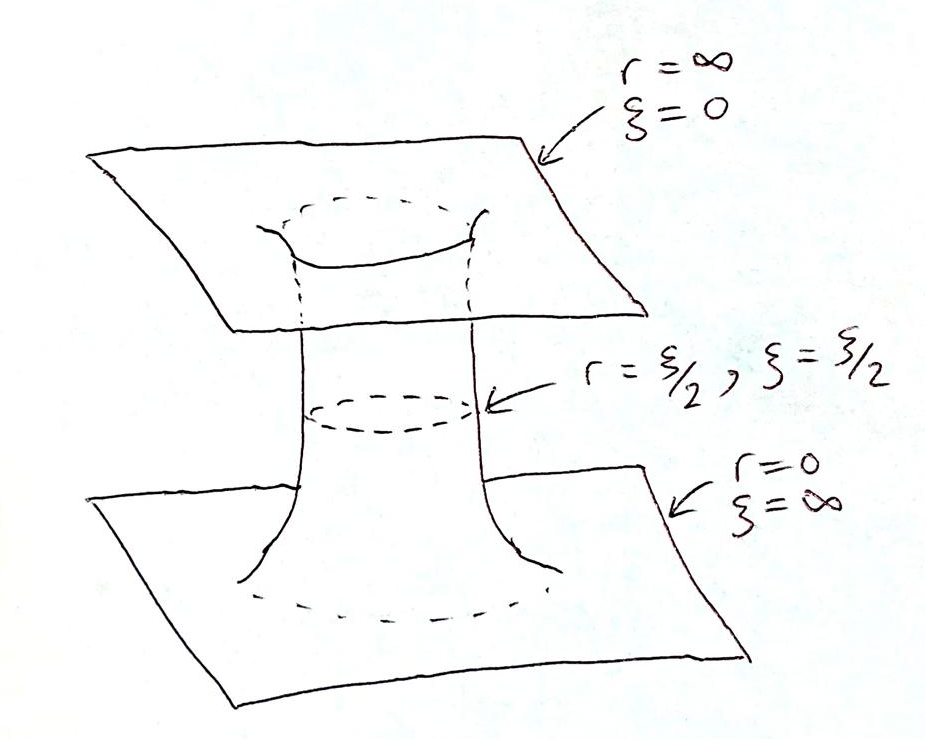
\includegraphics[width=0.6\textwidth]{png/scbh_er_bridge.png}
    \caption{Diagram to demonstrate the spacetime covered by isotropic coordinates. There are two asymptotically flat ends joined by the Einstein-Rosen bridge at $r=\xi=m/2$.}
    \label{intro:fig:scbh_er}
\end{figure}


\subsubsection{Penrose Diagrams and the Causal Structure of the Schwarzschild Black Hole}

NO9T SURE I NEED TO DISCUSS PENROSE DIAGRAMS HERE?


RANDOM TEXT RANDOM TEXT RANDOM TEXT RANDOM TEXT RANDOM TEXT RANDOM TEXT RANDOM TEXT RANDOM TEXT RANDOM TEXT RANDOM TEXT RANDOM TEXT RANDOM TEXT RANDOM TEXT RANDOM TEXT RANDOM TEXT RANDOM TEXT RANDOM TEXT RANDOM TEXT RANDOM TEXT RANDOM TEXT RANDOM TEXT RANDOM TEXT RANDOM TEXT RANDOM TEXT RANDOM TEXT RANDOM TEXT RANDOM TEXT RANDOM TEXT RANDOM TEXT RANDOM TEXT RANDOM TEXT RANDOM TEXT RANDOM TEXT RANDOM TEXT RANDOM TEXT RANDOM TEXT RANDOM TEXT RANDOM TEXT RANDOM TEXT RANDOM TEXT RANDOM TEXT RANDOM TEXT RANDOM TEXT RANDOM TEXT RANDOM TEXT RANDOM TEXT RANDOM TEXT RANDOM TEXT RANDOM TEXT RANDOM TEXT RANDOM TEXT RANDOM TEXT RANDOM TEXT RANDOM TEXT RANDOM TEXT RANDOM TEXT RANDOM TEXT RANDOM TEXT RANDOM TEXT RANDOM TEXT RANDOM TEXT RANDOM TEXT 

\begin{figure}[h!]
\centering
    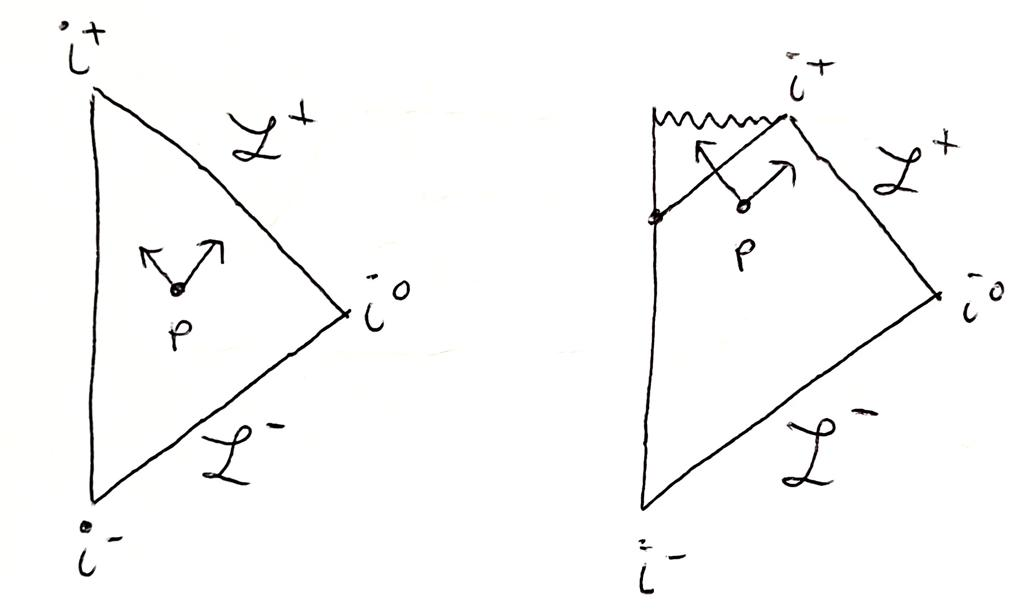
\includegraphics[width=0.65\textwidth]{png/penrose_mink.png}
    \caption{Diagram for proof of Penrose diagram of Minkowski space (left) and black hole formation from collapse (right). As shown from a point $p$, a null geodesic can fall into a black hole, but once inside can never return. }
    \label{intro:fig:scbh_penrose}
\end{figure}

RANDOM TEXT RANDOM TEXT RANDOM TEXT RANDOM TEXT RANDOM TEXT RANDOM TEXT RANDOM TEXT RANDOM TEXT RANDOM TEXT RANDOM TEXT RANDOM TEXT RANDOM TEXT RANDOM TEXT RANDOM TEXT RANDOM TEXT RANDOM TEXT RANDOM TEXT RANDOM TEXT RANDOM TEXT RANDOM TEXT RANDOM TEXT RANDOM TEXT RANDOM TEXT RANDOM TEXT RANDOM TEXT RANDOM TEXT RANDOM TEXT RANDOM TEXT RANDOM TEXT RANDOM TEXT RANDOM TEXT RANDOM TEXT RANDOM TEXT RANDOM TEXT RANDOM TEXT RANDOM TEXT RANDOM TEXT 

\begin{figure}[H]
\centering
    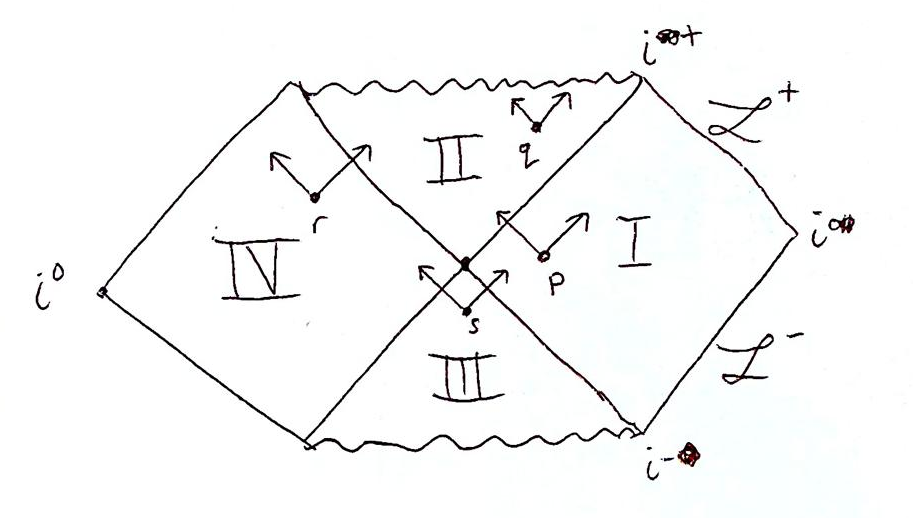
\includegraphics[width=0.65\textwidth]{png/scbh_penrose.png}
    \caption{Penrose diagram for the maximal extension of the Schwarzschild spacetime of the eternal black hole.}
    \label{intro:fig:scbh_penrose}
\end{figure}

RANDOM TEXT RANDOM TEXT RANDOM TEXT RANDOM TEXT RANDOM TEXT RANDOM TEXT RANDOM TEXT RANDOM TEXT RANDOM TEXT RANDOM TEXT RANDOM TEXT RANDOM TEXT RANDOM TEXT RANDOM TEXT RANDOM TEXT RANDOM TEXT RANDOM TEXT RANDOM TEXT RANDOM TEXT RANDOM TEXT RANDOM TEXT RANDOM TEXT RANDOM TEXT RANDOM TEXT RANDOM TEXT RANDOM TEXT RANDOM TEXT RANDOM TEXT RANDOM TEXT RANDOM TEXT RANDOM TEXT RANDOM TEXT RANDOM TEXT RANDOM TEXT RANDOM TEXT RANDOM TEXT RANDOM TEXT RANDOM TEXT 





\subsection{The Cosmological Constant} \label{intro:sec:cosmology}
A discussion of general relativity is incomplete without discussing the cosmological constant $\Lambda$. At a geometric level, the cosmological constant encodes the homogeneous spacetime curvature in the absense of matter, and indeed setting $\Lambda\rightarrow 0$ (in vacuum) returns asymptotically flat vacuum general relativity. The cosmological constant is added into Einstein's equation, Eq.~(\ref{intro:eq:einstein}), with a term like $\Lambda g_{\mu\nu}$,
\begin{equation} \label{intro:eq:einsteinlambda}
R_{\mu\nu}-\frac{1}{2}Rg_{\mu\nu}  +  \Lambda g_{\mu\nu} = \frac{8 \pi G}{c^4}T_{\mu\nu}.
\end{equation}
Each term still has a zero-divergence as $\nabla_\mu g_{\alpha\beta}=0$ due to the Levi-Civita connection defined in section \ref{intro:sec:levicivita}. The Einstein equation in vacuum becomes
\begin{equation}
R_{\mu\nu}-\frac{1}{2}Rg_{\mu\nu} + \Lambda g_{\mu\nu} = 0,
\end{equation}
and the traced becomes
\begin{equation}
R = \frac{2D}{D-2}\Lambda
\end{equation}
for $D$ spacetime dimensions. This quite nicely shows us that in the limit $\Lambda=0$ the normal vacuum GR solution $R=0$ is returned. In the case $\Lambda\neq 0$ it describes a homogeneous curved universe with constant non-zero $R$.

\subsubsection*{Friedmann–Lemaître–Robertson–Walker Spacetime}

To model the entire universe more realistically, an isotropic uniform fluid as added. A uniform matter distribution is often done with a perfect fluid with stress tensor,
\begin{equation}
T_{\mu\nu} = (\rho+P)u_\mu u_\nu + Pg_{\mu\nu},
\end{equation}
where $\rho$ and $P$ are the rest frame density and pressure. The fluid is taken to be at rest with $u^i =0$ and $\bs{g}(\bs{u},\bs{u})=-1$. The line element takes the following ansatz,
\begin{equation}
\dd s^2 = -\dd t^2 + a^2(t) \gamma_{ij} \dd x^i \dd x^j,
\end{equation}
where $a(t)$ is the scale factor of the universe and the spacelike metric $\bs{\gamma}$ is given by,
\begin{align}
\gamma_{ij} \dd x^i \dd x^j = 
\Bigg\{
\begin{array}{ll}
{\dd r^2} + \sin^2(r) \left(\dd \theta^2 + \sin^2(\theta) \dd \phi^2 \right)\quad&, \,\,\,(\mathrm{closed}) \\
\dd r^2 + r^2 \left(\dd \theta^2 + \sin^2(\theta) \dd \phi^2 \right)\,\quad\quad&, \,\,\,(\mathrm{flat}) \\
{\dd r^2} + \sinh^2(r) \left(\dd \theta^2 + \sin^2(\theta) \dd \phi^2 \right)&, \,\,\,(\mathrm{hyperbolic} ) 
\end{array}
\end{align}
for either uniformly curved hyperbolic space, uniformly curved closed space or flat space. This spacetime is called the Friedmann–Lemaître–Robertson–Walker spacetime and the trace of Eintein's equation in four dimensions becomes,
\begin{equation}
R = 4\Lambda -8\pi T,
\end{equation}
where planck units are used and $T=T_{\mu\nu}g^{\mu\nu}$. It should be noted that $R$ and $T$ are constant over the entire spatial domain of the spacetime for a moment of time. This form of Einstein's equation makes it abundantly clear that the cosmological constant has the same effect on curvature as a uniform matter distribution. In the case $4 \Lambda = 8 \pi T$, Einstein's equation is once again $R=0$ and can be solved with the flat metric of Minkowski (but now it is not in vacuum unless $T=\Lambda=0$). If $8\pi T> 4\Lambda$, then the spatial hypersurface of the universe is closed and finite sized. Finally, if $4\Lambda > 8 \pi T$ then the spatial hypersurface of the universe is open or hyperbolic; as a radial geodesics is followed, the amount of space grows faster than the $r^2$ as expected in flat space.

Putting the ansatz for the metric and stress tensor into the Einstein equation returns an ODE for $a(t)$. Along with an equation of state, $P(\rho)$, the continuity equation $\nabla_\mu T^{\mu\nu}=0$ returns an ODE for $\rho(t)$. The two solutions $\rho(t)$ and $a(t)$, along with knowledge of whether the spatial time-slices are flat, closed or hyperbolic, fully specify the spacetime. These solutions cover many topics such as the big bang, inflation, universe expansion, bouncing cosmologies (ending with a big crunch) and also minkowksi space given the correct conditions. 



\subsection{The Lagrangean Formulation of General Relativity}\label{intro:sec:gr_from_lagrangean}
A common procedure in theoretical physics is to encapsulate the solution space in an action functional $S$,
\begin{equation}
S = \int \mathcal{L} \sqrt{-g} \,\dd x^4.
\end{equation}
Using the calculus of variation on this action returns differential equations governing the system. As found by Hilbert [REF] the following lagrangean density $\mathcal{L}=R$, equal to the Ricci scalar, returns the vacuum Einstein equations under varying with respect to $g^{\mu\nu}$.
\begin{align}
\delta S &= \int \left[\sqrt{-g} (\delta R) + R (\delta \sqrt{-g})\right]\,\dd x^4 \\
&= \int \left[\sqrt{-g} \delta(g^{\mu\nu}R_{\mu\nu}) -\frac{1}{2} \sqrt{-g} g_{\mu\nu}R (\delta g^{\mu\nu})\right]\,\dd x^4 \\
&= \int \left[\sqrt{-g}g^{\mu\nu}(\delta R_{\mu\nu}) + \sqrt{-g}\left(R_{\mu\nu}-\frac{1}{2}R g_{\mu\nu} \right)\delta g^{\mu\nu}\right]\,\dd x^4 \label{intro:eq:varric}
\end{align}  
where we used Eq.~(\ref{intro:eq:gdggdg}) to vary $\sqrt{-g}$. Remembering that the difference of two christoffel symbols such as,
\begin{equation}
\delta \Gamma^{\lambda}_{\,\,\,\mu\nu} = \Gamma^{\lambda}_{\,\,\,\mu\nu}|_{g^{\mu\nu}+\delta g^{\mu\nu}} - \Gamma^{\lambda}_{\,\,\,\mu\nu}|_{g^{\mu\nu}}
\end{equation} 
is a tensor, and using normal coordinates discussed in section \ref{intro:sec:normal_coords} the left hand term of Eq.~(\ref{intro:eq:varric}) becomes
\begin{align}
g^{\mu\nu} \delta R_{\mu\nu} &= g^{\mu\nu}\left( \partial_\lambda \delta\Gamma^{\lambda}_{\,\,\,\mu\nu} - \partial_\nu \delta\Gamma^{\lambda}_{\,\,\,\mu\lambda} \right), \\
&= g^{\mu\nu}\left( \nabla_\lambda \delta\Gamma^{\lambda}_{\,\,\,\mu\nu} - \nabla_\nu \delta\Gamma^{\lambda}_{\,\,\,\mu\lambda} \right), \\
&= \nabla_\lambda \left( g^{\mu\nu} \delta\Gamma^{\lambda}_{\,\,\,\mu\nu} - g^{\mu\lambda} \delta\Gamma^{\nu}_{\,\,\,\mu\nu} \right), \\
&=\nabla_\lambda X^\lambda.
\end{align}
The ability to transform the partial derivatives into covariant derivatives comes from using normal coordinates. Putting everything together, $\delta S$ becomes
\begin{align}
\delta S &= \int \left[ \nabla_\mu X^\mu + \left( R_{\mu\nu}-\frac{1}{2}Rg_{\mu\nu}\right)\right]\sqrt{-g}\,\dd x^4, \\
&= \int_B X^\mu \hat{s}_\mu \sqrt{|{}^{(3)}g|}\dd x^3 + \int \left[  R_{\mu\nu}-\frac{1}{2}Rg_{\mu\nu}\right]\sqrt{-g}\,\dd x^4, \\
\end{align}
where the integral over $B$ represents the surface integral over the boundary of our spacetime with metric ${}^{(3)}g_{ij}$; on B $\delta g^{\mu\nu}\rightarrow 0 $ and therefore $X^\mu \rightarrow 0$. Setting $\dd S =0$ implies
\begin{equation}
R_{\mu\nu}-\frac{1}{2}Rg_{\mu\nu}=0,
\end{equation} 
which is the vacuum Einstein equation.

\subsubsection*{Non-Vacuum Spacetimes}
Matter is often added into a spacetime at the level of the lagrangean with a term $\frac{16 \pi G}{c^4}\L_m$. The cosmological constant can be added in exactly the same way with $\L_\Lambda$. The total lagrangean becomes,
\begin{equation}
S = \int \left({R} + \frac{16 \pi G}{c^4} \L_m + \L_\Lambda \right)\sqrt{-g} \,\dd x^4.
\end{equation}
As we have already seen earlier in this section, the variation of $R$ with respect to the inverse metric components $g^{\mu\nu}$ returns the vacuum Einstein equation; adding the two new terms from $\L_m$ and $\L_\Lambda$, setting $\delta S =0$ gives different equation
\begin{equation}
R_{\mu\nu} - \frac{1}{2}Rg_{\mu\nu} + \frac{16 \pi G}{c^4}\frac{1}{\sqrt{-g}}\frac{\delta( \L_m \sqrt{-g})}{\delta g^{\mu\nu}} + \frac{1}{\sqrt{-g}}\frac{\delta (\L_\Lambda \sqrt{-g})}{\delta g^{\mu\nu}} = 0.
\end{equation}
Comparing the $\L_\Lambda$ term to the Einstein equation with cosmological constant in Eq.~(\ref{intro:eq:einsteinlambda}) we must have
\begin{align}
g_{\mu\nu} \Lambda &= \frac{1}{\sqrt{-g}}\frac{\delta (\L_\Lambda \sqrt{-g})}{\delta g^{\mu\nu}} , \\
&= \L_\Lambda \frac{1}{\sqrt{-g}}\frac{\delta ( \sqrt{-g})}{\delta g^{\mu\nu}} + \frac{\delta (\L_\Lambda )}{\delta g^{\mu\nu}}, \\
&=-\frac{1}{2}g_{\mu\nu}\L_\Lambda  + \frac{\delta (\L_\Lambda )}{\delta g^{\mu\nu}}, \\
\end{align}
which is solved by $\L_\Lambda = -2\Lambda$. Comparing the matter term instead returns another definition of the stress tensor,
\begin{align}
T_{\mu\nu}:&=-\frac{2}{\sqrt{-g}}\frac{\delta (\L_m \sqrt{-g})}{\delta g^{\mu\nu}},\\
&= -2\frac{\delta \L_m}{\delta g^{\mu\nu}} + g_{\mu\nu} \L_m .\label{intro:eq:Tdef}
\end{align} 
Collecting these results, the full lagrangean is,
\begin{align}
\L = R + \frac{16 \pi G}{c^4} \L_m -2\Lambda,
\end{align}
or in Planck units,
\begin{align}
\L = R + 16 \pi \L_m -2\Lambda.
\end{align}
The form of $\L_m$ is problem specific, depending on the type of matter. The equation of motion of the matter, described by a set of fields $\phi_i$, and their partial derivatives with respect to $x^\mu$ is,
\begin{equation}
\sqrt{-g}\frac{\delta \L}{\delta \phi_i} -\partial_\mu \left(\sqrt{-g}\frac{\delta\L}{\delta \partial_\mu \phi_i}\right)=0.
\end{equation}
If the $\phi_i$ are scalar fields then the equation of motion simplifies, using Eq.~(\ref{intro:eq:div_vector}), to 
\begin{equation}
\frac{\delta \L}{\delta \phi_i} - \nabla_\mu \left(\frac{\delta\L}{\delta \nabla_\mu \phi_i}\right)=0.
\end{equation}

\subsubsection*{Modified Theories of Gravity}

The Lagrangean formulation of general relativity is especially useful for the more theoretical apects of general relativity such as exotic matter and modified gravity. General relativity is not thought of as the "correct" or "final" theory of gravity. It is a classical field theory so cannot describe particles or quantum mechanics. To date no sucessful quantisation of general relativity has been done. Another problem with general relativity is that at the centre of black holes there are singularities; a similar singularity exists for the Coulomb force of a point particle. The Coulomb force singularity is resolved by quantum field theory (QFT); it is thought a similar thing may happen in a quantum field theory for gravity but it is currently unknown.

Theories such as string theory and loop quantum gravity have attempt to describe a quantum theory of gravity but are notoriously difficult to derive observable effects from. Many modified gravity theories aim to describe the first deviation from general relativity towards a quantum gravity. It is thought that deviations from general relativity might be seen in extremely high curvature regimes.


Currently there is no conclusive experimental evidence of deviations from general relativity.

At the level of the lagrangean, minimal coupling means to write down the simplest lagrangean possible - without coupling between matter fields and Ricci curvature. As an example, the action for the minimally coupled scalar field $\psi$ in curved space is,
\begin{equation}
S_\psi = \int \left( aR - b g^{\mu\nu}\partial_\mu \psi \partial_\nu \psi \right) \sqrt{-g}\,\dd^4 x,
\end{equation}
for constants $a$ and $b$. Extra coupling terms between matter and curvature could be added, for instance the action,
\begin{equation}
S_f = \int \left( aRf(\psi) - b g^{\mu\nu}\partial_\mu \psi \partial_\nu \psi \right) \sqrt{-g}\,\dd^4 x,
\end{equation}
for some function $f$; note that if $f$ is constant then this action is the minimally coupled wave sf asdf. Varying $S_f$ with respect to $g^{\mu\nu}$ gives a modified Einstein equation,
\begin{equation}
f(\psi) R_{\mu\nu} - \frac{1}{2} R f(\psi)g_{\mu\nu} + R \frac{\delta f}{\delta g^{\mu\nu}}(\psi) = \frac{b}{a} \left(\nabla_\mu \psi \nabla_\nu \psi-\frac{1}{2} g_{\mu\nu} g^{\rho\sigma}\nabla_\rho \psi \nabla_\sigma\psi  \right), 
\end{equation}
where a new type of term $ R \frac{\delta f}{\delta g^{\mu\nu}}(\psi)$ coupling gravity and matter has arisen; note this becomes the regular Einstein equation for a spacetime with a real massless scalar field $\psi$ if $f$ is constant. Varying $S_f$ with respect to $\psi$ instead gives the modified wave equation,
\begin{equation}
g^{\mu\nu}\nabla_\mu \nabla_\nu \psi + \frac{a}{b}R \frac{\partial f}{\partial \psi} =0,
\end{equation}
which is equivalent to Eq.~(\ref{intro:eq:modified_wave}); note that this returns the regular curved space wave equation if $\partial f / \partial \psi=0$ and the regular wave equation in the flat-space limit.

other popular methods of modifying gravity include higher poowers of curvature such as the gauss bonnet ...

\subsection{STUFF}

finish modified gravity and a lightnight fast introduction to penrose diagrms (probably onyl mention krustal skzeres coords or ref them?)



% \section{Might Delete}

% \subsection{Differential Forms - MIGHT DELETE}
% A differential $p$-form is an antisymetric $(0,p)$ tensor; the tensor components (e.g. $A_{\alpha\beta...\zeta}$) vanish if there is a repeating index, equal $1$ for an even permutation of indeces (like 1,2,3,...,N) and $-1$ for an odd permutation (such as 2,1,3,4,...,N). Note that a $0$-form is a function, a $1$-form is a co-vector and for an $N$-dimensional manifold the $N$-form is unique and the $p$-forms with $p>N$ vanish. 

% When considering differential forms, the conventional covector basis is often changed from $\bs{\theta}^\mu$ to $\dd x^\mu$ which will lend itself nicely to integrating p-forms on manifolds later. This convention means we can write the metric as $\bs{g} = g_{\mu\nu} \dd x^\mu \otimes \dd x^\nu$; the same can be done for any tensor. Note that the metric cannot be a $2$-form as it is not a symmetric tensor, infact the metric is a symmetric tensor.

% Differential forms have their own unique differential operator called the exterior derivative, it acts on a p-form and returns a $p+1$-form. For a $p$-form $\bs{A} = A_\mu \dd x^\mu$, the exterior derivative is given by 
% \begin{equation}
% (\dd A)_{\mu_1 ... \mu_{p+1}} = (p+1)\partial_{[ \mu_1}A_{\mu_2 ... \mu_{p+1}]},
% \end{equation}
% where the square brackets mean the antisymmetric [check as i might need epsilons here ]. This derivative guarentees to return a tensor without the need for a connection or metric on the manifold, unlike the partial derivative that we will see next. One common example of an exterior derivative is of a 1-form, say $\bs{A}$, giving 
% \begin{equation}
% (\dd A)_{\mu\nu} = \partial_\mu A_\nu - \partial_\nu A_\mu,
% \end{equation}
% which returns a 2-form. To be a 2-form the tensor must be antisymmetric under swapping indeces like $(\dd A)_{\mu\nu} = -(\dd A)_{\nu\mu}$, which is trivially true, and must transform like a tensor. Performing a coordinate transformation on $(\dd A)_{\mu\nu}$ we see it transforms like 
% \begin{align}
% \frac{\partial}{\partial \tilde{x}^\mu}\tilde{A}_\nu - \frac{\partial}{\partial \tilde{x}^\nu} \tilde{A}_\mu &= 
% \frac{\partial x^\rho}{\partial \tilde{x}^\mu}\frac{\partial}{\partial {x}^\rho}\left(\frac{\partial {x}^\sigma}{\partial\tilde{x}^\nu}A_\sigma\right) 
% - \frac{\partial x^\sigma}{\partial \tilde{x}^\nu}\frac{\partial}{\partial {x}^\sigma}\left(\frac{\partial {x}^\rho}{\partial\tilde{x}^\mu}A_\rho\right) ,\\
% &= \frac{\partial x^\rho}{\partial \tilde{x}^\mu}\frac{\partial {x}^\sigma}{\partial\tilde{x}^\nu}\left(\frac{\partial}{\partial {x}^\rho} A_\sigma - \frac{\partial}{\partial {x}^\sigma} A_\rho\right)
% + 
% \frac{\partial x^\rho}{\partial \tilde{x}^\mu}\frac{\partial}{\partial {x}^\rho}\left(\frac{\partial {x}^\sigma}{\partial\tilde{x}^\nu}\right) A_\sigma
% - \frac{\partial x^\sigma}{\partial \tilde{x}^\nu}\frac{\partial}{\partial {x}^\sigma}\left(\frac{\partial {x}^\rho}{\partial\tilde{x}^\mu}\right)A_\rho ,\\
% &= \frac{\partial x^\rho}{\partial \tilde{x}^\mu}\frac{\partial {x}^\sigma}{\partial\tilde{x}^\nu}\left(\frac{\partial}{\partial {x}^\rho} A_\sigma - \frac{\partial}{\partial {x}^\sigma} A_\rho\right)
% + 
% \left(  \frac{\partial^2 {x}^\rho}{\partial \tilde{x}^\mu\partial\tilde{x}^\nu} 
% - \frac{\partial^2 {x}^\rho}{\partial\tilde{x}^\nu\partial\tilde{x}^\mu} \right)A_\rho ,\\
% &= \frac{\partial x^\rho}{\partial \tilde{x}^\mu}\frac{\partial {x}^\sigma}{\partial\tilde{x}^\nu}\left(\frac{\partial}{\partial {x}^\rho} A_\sigma - \frac{\partial}{\partial {x}^\sigma} A_\rho\right),
% \end{align}
% which is exactly the tensor transformation law.

% COVER HER THAT DD GIVES ZERO?
% HODGE ? REWRITE DIFF EQNS WITH FORM NOTATION AND HODGE THEORY?
% PROVE 




% \subsection{Parallel Transport - MIGHT DELETE}


% Parallel transport is the procedure of moving tensors along a smooth curve in a manifold. The curve $\Gamma$ can be expressed parametrically as $x^\mu(\tau)$ with respect to a parameter $\tau$, this automatically gives us the tangent vector $\bs{X}$ to $\Gamma$ like 
% \begin{equation}
% X^\mu(\tau) = \frac{\partial x^\mu(\tau)}{\partial \tau} = \dot{x}^\mu.
% \end{equation}
% Parallel transporting a tensor $\bs{T}$ along $\Gamma$ requires that $\bs{\nabla}_{\bs{X}} \bs{T}$ must be satisfied along $\Gamma$ where $\bs{\nabla}_{\bs{X}}=x^\mu \nabla_\mu$.

% MAYBE DO THE FAMOUS VECTOR ON A SPHERE EXAMPLE

% Having discussed parallel transport, we can re-derive geodesics. Take a vector field $\bs{X}$ and parallel transport is along it's own integral curves, therefore $\bs{X}$ must satisfy $\bs{\nabla}_{\bs{X}}\bs{X}=0$. With a little algebra we can show that this describes a geodesic,
% \begin{align}
% x^\mu \nabla_\mu X^\nu &=0, \\
% x^\mu \nabla_\mu X^\nu &= X^\mu \partial_\mu X^\nu + X^\mu \Gamma^{\nu}_{\,\,\,\rho\mu}X^\rho, \\
% &=\frac{\partial x^\mu(\tau)}{\partial \tau}\frac{\partial}{\partial x^\mu} \frac{\partial x^\nu(\tau)}{\partial \tau} + \Gamma^{\nu}_{\,\,\,\rho\mu}\frac{\partial x^\mu(\tau)}{\partial \tau}\frac{\partial x^\rho(\tau)}{\partial \tau},\\
% &=\frac{\partial}{\partial \tau} \frac{\partial x^\nu(\tau)}{\partial \tau} + \Gamma^{\nu}_{\,\,\,\rho\mu}\frac{\partial x^\mu(\tau)}{\partial \tau}\frac{\partial x^\rho(\tau)}{\partial \tau},\\
% \label{intro:eq:geo}&= \ddot{x}^\nu + \Gamma^{\nu}_{\,\,\,\rho\mu}\dot{x}^\rho\dot{x}^\mu
% \end{align}
% and we have re-derived Eq.~(\ref{intro:eq:geodesic}). Again this aligns with our intuition of a geodesic in flat space. We already remarked in Section \ref{intro:sect:lgm} that $\ddot{x}^\mu=0$ describes a straight line in flat space (when using cartesian coordinates) and now we can add another interpretation; in flat space a geodesic (which is a straight line) can be created by transporting a vector along it's own direction.


% \subsection{Low Curvature Limit of General Relativity - MIGHT DELETE}
% An important use of General Relativity is it's use in the low curvature limit. The simplest example of this would be Special Relativity; if General Relativity i[DO] reproduce Special Relativity in the limit of vanishing curvature then it is. We work with the assumption of a vacuum spacetime with no Cosmological constant and seek solutions to the Einstein equation with metric $g_{\mu\nu} = \eta_{\mu\nu}$ where 
% \begin{equation}
% \eta_{\mu\nu} = \begin{pmatrix} -1 & 0 & 0 & 0 \\ 0 & 1 & 0 & 0 \\ 0 & 0 & 1 & 0 \\ 0 & 0 & 0 & 1 \\\end{pmatrix}
% \end{equation}
% in Cartesian coordinates. As seen before, in Eq.[REF]REF the Einstein equation in vacuum simplfies to just a vanishing Ricci tensor,
% \begin{align} \label{intro:eq:ricc=0}
% R_{\mu\nu} &= 0 ,\\
%            &= \partial_{\rho}\Gamma^{\rho}_{\,\,\,\mu \nu}-\partial_{\nu}\Gamma^{\rho}_{\,\,\,\mu \rho} + \Gamma^{\rho}_{\,\,\, \rho\sigma}\Gamma^{\sigma}_{\,\,\,\mu \nu}-\Gamma^{\rho}_{\,\,\,\mu \sigma}\Gamma^{\sigma}_{\,\,\, \rho\nu}.
% \end{align}
% Given that the Connection symbols $\Gamma^\mu_{\,\,\,\nu\rho}$ vanish everywhere for the metric components ${\eta}_{\mu\nu}$ then Eq.~(\ref{intro:eq:ricc=0}) is trivially satisfied and we have proved that Special Relativity is the zero-curvature limit of GR.

% Relaxing the condition $g_{\mu\nu}=\eta_{\mu\nu}$ to $g_{\mu\nu}=\eta_{\mu\nu}+h_{\mu\nu}$, where the components $h_{\mu\nu} \ll 1$, we can create a vacuum spacetime consisting of small curvature fluctuations; this turns out to describe gravitational waves. Ignoring terms of order $\mathcal{O}(h^2)$ we can see that
% \begin{align}
% g^{\mu\nu} &= \eta^{\mu\nu} - h^{\mu\nu}, \\
% h^{\rho\sigma} &= \eta^{\mu\rho}\eta^{\nu\sigma}h_{\mu\nu},\\
% g^{\mu\nu}g_{\nu\rho} &= \delta^\mu_\rho =\eta^{\mu\nu}\eta_{\nu\rho} +\eta^{\mu\nu}h_{\nu\rho} - h^{\mu\nu}\eta_{\nu\rho} + \mathcal{O}(h^2),\\
%                       &= \delta^\mu_\rho +\eta^{\mu\nu}h_{\nu\rho} - \eta^{\mu\alpha}\eta^{\nu\beta} h_{\alpha\beta}\eta_{\nu\rho},\\
%                       &= \delta^\mu_\rho +\underbrace{\eta^{\mu\nu}h_{\nu\rho} - \eta^{\mu\alpha} h_{\alpha\rho}}_{=0}.
% \end{align}
% Note that we raise/lower the indeces of $h_{\mu\nu}$/$h^{\mu\nu}$ with $\bs{\eta}$ and not $\bs{g}$ THIS IS WRONG. Looking at the connection symbols and Ricci tensor while ignoring $\mathcal{O}(h^2)$ terms we get
% \begin{align}
% \Gamma^{\rho}_{\,\,\,\mu\nu} &= \frac{1}{2}\left(\eta^{\rho\sigma}-h^{\rho\sigma}\right)\left( \partial_\mu(\eta_{\sigma\nu}+h_{\sigma\nu}) + \partial_\nu(\eta_{\mu\sigma}+h_{\mu\sigma})-\partial_\sigma(\eta_{\mu\nu}+h_{\mu\nu}) \right),\\
%                              &=\frac{1}{2}\eta^{\rho\sigma}\left( \partial_\mu h_{\sigma\nu} + \partial_\nu h_{\mu\sigma}-\partial_\sigma h_{\mu\nu} \right) + \mathcal{O}(h^2),\\
%                   R_{\mu\nu}& = \partial_{\rho}\Gamma^{\rho}_{\,\,\,\mu \nu}-\partial_{\nu}\Gamma^{\rho}_{\,\,\,\mu \rho} + \mathcal{O}(h^2),\\
%                             & = \frac{1}{2}\eta^{\rho\sigma}\left( \partial_\rho \partial_\mu h_{\sigma\nu} - \partial_\rho \partial_\sigma h_{\mu\nu}  - \partial_\nu \partial_\mu h_{\sigma\rho} +  \partial_\sigma \partial_\mu h_{\rho\mu} \right) +\mathcal{O}(h^2),\\
%                         R=& ({\eta^{\mu\nu}-h^{\mu\nu}})R_{\mu\nu},\\
%                           &= \eta^{\mu\nu}\eta^{\rho\sigma}(\partial_\mu \partial_\rho h_{\sigma \nu} - \partial_\sigma \partial_\rho h_{\mu\nu}) +\mathcal{O}(h^2).
% \end{align}
% To simplify the solving of Einsteins eqn [FIX THIS] we can consider coordinate transformation like $x^\mu \rightarrow x^\mu + \zeta^\mu$ where $\zeta^\mu\ll1$. It can easily be shown that to first order in $\zeta^\mu$ and $h_{\mu\nu}$ that $h_{\mu\nu}$ transforms like 
% \begin{equation}
% h_{\mu\nu} \rightarrow h_{\mu\nu} + \partial_{\mu}\zeta_\nu + \partial_\nu \zeta_\mu
% \end{equation} 
% where raising/lowering the indeces of $\bs{\zeta}$ is done with $\bs{\eta}$ as terms of order $\mathcal{O}(h)\mathcal{O}(\zeta)$ are ignored.


% Note [TALK ABOUT G PLUS H RATHER THAN ETA PLUS H FOR BH RINGDOWN AND MAYBE BS STABILITY? THIS IS MORE PERTURBATION THEORY THOUGH]




% [MENTION : GW'S, PRECESSION, LIGHT DEFLECTION, TIME DILATION AROUND EARTH/SUN, MAYBE MENTION INTERSTELLAR'S TIME DILATION? ARE THESE REALLY LOW ENERGY LIMIT? MENTION POST NEWTONIAN OTHER THINGS?]



